% !Mode:: "Tex:UTF-8"

El último capítulo de esta parte del curso marca el inicio de la transición hacia los temas de los
que nos vamos a ocupar de aquí hasta el final. En todos los problemas de inferencia que hemos
estudiado hasta ahora, hemos supuesto que nuestro interés se reducía a una única población. Sin
embargo, en las aplicaciones de la Estadística, a menudo nos encontramos con situaciones en las que
lo natural es comparar los datos procedentes de varias poblaciones, {\em precisamente para ver si
existen diferencias entre ellas.} Por ejemplo, con los métodos del Capítulo
\ref{cap:IntervalosConfianza} estamos preparados para estimar (mediante un intervalo de confianza)
la longevidad media de los españoles. Pero para situarla en su contexto, seguramente querríamos
compararla con la longevidad media de franceses, japoneses, rusos, etc. Ese sería un problema
típico en el que querríamos comparar las medias de una misma variable (la longevidad) en distintas
poblaciones. En otros problemas querríamos comparar proporciones, o varianzas, o cualquier otro
parámetro de una misma variable, en las poblaciones que nos interesan. En este capítulo vamos a
estudiar el primero, por ser el más sencillo, de estos problemas, en el que se trata de comparar
{\em precisamente dos poblaciones}. En la última parte del curso, y dentro del contexto general de
la relación entre variables aleatorias, veremos como generalizar los métodos de este capítulo a un
número cualquiera de poblaciones. No obstante, veremos que al comparar, por ejemplo, cuatro
poblaciones, a veces es necesario o conveniente realizar todas las comparaciones dos a dos de esas
cuatro poblaciones (un total de $\binom{4}{2}=6$ comparaciones). Aunque sólo fuera por esa razón,
es imprescindible empezar estudiando el caso especial de dos poblaciones, al que recurriremos más
adelante.

Empezaremos por el problema de comparar dos proporciones, seguiremos con las medias y terminaremos
comparando varianzas. Es un capítulo denso en fórmulas nuevas, pero las ideas básicas (intervalos,
contrastes) ya nos resultan conocidas. Por eso, antes de empezar, queremos hacer una advertencia.
Es bueno adquirir una cierta {\em familiaridad} con las fórmulas de este capítulo, pero estamos
convencidos de que, para la inmensa mayoría de los lectores, memorizarlas es una pérdida de tiempo
y de esfuerzo.

\section{Diferencia de proporciones en dos poblaciones.}
\label{cap09:sec:DiferenciaProporciones2Poblaciones}

Para seguir la estela del capítulo previo, vamos a empezar por el problema de comparar la
proporción de individuos de dos poblaciones que presentan cierta característica, la misma en ambas
poblaciones. Los ejemplos de este tipo de problemas son numerosos: un nuevo tratamiento que se
prueba en dos grupos, mediante ensayos de tipo doble ciego, administrando el tratamiento a un grupo
y un placebo al grupo de control. Lo que nos interesa es, por ejemplo, saber si la proporción de
pacientes que experimentan mejoría es la misma en ambos grupos. En otro ejemplo tenemos dos
poblaciones de una misma especie de árboles, y queremos estudiar si la proporción de entre ellas
que están infectadas con un determinado hongo es distinta. Podríamos seguir con otros muchos
ejemplos, pero lo que todos ellos tienen en común es que:
\begin{enumerate}
            \item tenemos dos poblaciones (que llamaremos población 1 y población 2), y una misma
                variable aleatoria, definida en ambas poblaciones. Esa variable representa la
                proporción de individuos de cada población que presentan una determinada
                característica. Se trata por tanto de una variable de tipo Bernouilli, pero el
                parámetro $p$ (la proporción) puede ser distinto en las dos poblaciones. Así que
                tenemos que usar dos símbolos, $p_1$ y $p_2$, para referirnos a las proporciones
                en cada una de las poblaciones.
            \item Tomamos dos muestras aleatorias, una en cada población, de tamaños $n_1$ y
                $n_2$ respectivamente. Y para cada una de esas muestras calculamos la proporción
                muestral; se obtendrán, de nuevo, dos valores
                \[\hat p_1=\dfrac{X_1}{n_1}\quad \mbox{ y }\quad \hat p_2=\dfrac{X_2}{n_2},\]
                Siendo $X_1$ y $X_2$, respectivamente, el número de éxitos en cada muestra. Las
                muestras son, desde luego, independientes.
            \item El objetivo de nuestro estudio es comparar ambas proporciones, analizando la diferencia $p_1-p_2$. Y, como en secciones precedentes, lo que queremos es obtener intervalos de confianza para $p_1-p_2$, y poder realizar contrastes de hipótesis sobre esa diferencia.
\end{enumerate}
Una vez planteado el problema, los pasos que hay que dar son los que ya hemos visto en situaciones
previas. Sabemos que necesitamos un estadístico que relacione $(p_1-p_2)$ con los valores de las
muestras ($n_1, n_2, \hat p_1, \hat p_2$), y cuya distribución de probabilidades sea conocida. Para
obtener ese estadístico, vamos a imponer alguna condición a la distribución de la variable en las
dos poblaciones.

En concreto vamos a suponer, para empezar, que ambas muestras son suficientemente grandes, y que $\hat p_1$ y $\hat p_2$ no son demasiado pequeñas (ni demasiado cercanas a $1$). Es decir, que se cumplen todas estas condiciones
    \[n_1>30,\quad n_2>30, \quad n_1\cdot\hat p_1>5,\quad n_1\cdot\hat q_1>5,\quad  n_2\cdot\hat p_2>5,\quad n_2\cdot\hat q_2>5.\]
Entonces las dos poblaciones se comportan aproximadamente como las normales
\[X_1\sim N(n_1p_1,\sqrt{n_1p_1q_1})\quad \mbox{ y }\quad X_2\sim N(n_2p_2,\sqrt{n_2p_2q_2}),\]
respectivamente. A partir de esta información, obtenemos la información necesaria sobre la
distribución muestral de la diferencia $\hat p_1-\hat p_2$. Vimos, en el Capítulo
\ref{cap:DistribucionesRelacionadasBinomial}, (pág. \pageref{cap08:ecu:EstadisticoProporciones}),
que en estas condiciones las proporciones muestrales tienen una distribución muy parecida a la de
una normal, concretamente:
    \[\hat p_1\sim N\left(p_1,\sqrt{\dfrac{\hat p_1\cdot\hat q_1}{n_1}}\right)\qquad\mbox{ y, análogamente, }\qquad \hat p_2\sim N\left(p_2,\sqrt{\dfrac{\hat p_2\cdot\hat q_2}{n_2}}\right).\]
Eso significa que la diferencia $\hat p_1-\hat p_2$ se parece (mucho) a la diferencia de dos
distribuciones normales, que son independientes puesto que lo son las muestras. Y, recordando lo
que vimos en la Ecuación \ref{cap05:ecu:SumaVariablesNormalesIndependientes} (pág.
\pageref{cap05:ecu:SumaVariablesNormalesIndependientes}) sobre la suma de variables normales
independientes,  eso significa que la diferencia se puede aproximar ella misma por una normal. A
partir de esto, el camino para obtener el estadístico adecuado está despejado:
\begin{center}
    \fcolorbox{black}{Gris025}{
    \begin{minipage}{12.5cm}
        %%%%%%%%%%%%%%%%%%%%%%%%%%%%%%%%%%%%%%%
        \begin{center}
        {\bf Estadístico para la diferencia de proporciones.}
        \index{estadístico para la diferencia de proporciones}
        \end{center}
       %%%%%%%%%%%%%%%%%%%%%%%%%%%%%%%%%%%%%%%
        Si se cumplen las condiciones
            \begin{equation}
            %\label{cap09:ecu:CondicionesAproximacionBinomialNormalDosMuestras}
            \label{cap09:ecu:CondicionesInferenciaDiferenciaProporciones}
            %n_1>30,\quad  n_2>30,\quad  n_1\cdot\hat p_1>5,\quad n_1\cdot\hat q_1>5, \quad n_2\cdot\hat p_2>5,\quad n_2\cdot\hat q_2>5,
                \begin{cases}
                n_1>30,\quad n_2>30,\\
                n_1\cdot\hat p_1>5,\quad n_1\cdot\hat q_1>5,\\
                n_2\cdot\hat p_2>5,\quad n_2\cdot\hat q_2>5,
                \end{cases}
            \end{equation}
        entonces la diferencia de proporciones se puede aproximar por esta distribución normal:
            \[\hat p_1-\hat p_2\sim N\left(p_1-p_2,\sqrt{\dfrac{\hat p_1\cdot\hat q_1}{n_1}+\dfrac{\hat p_2\cdot\hat q_2}{n_2}}\right)\]
        Por lo tanto el estadístico:
            \begin{equation}\label{cap09:ecu:EstadisticoDiferencia2Proporciones}
                \dfrac{\left(\hat p_1-\hat p_2\right)-\left(p_1-p_2\right)}{\sqrt{\dfrac{\hat p_1\cdot\hat q_1}{n_1}+\dfrac{\hat p_2\cdot\hat q_2}{n_2}}}
            \end{equation}
        tiene una distribución normal estándar $N(0,1)$.
       %%%%%%%%%%%%%%%%%%%%%%%%%%%%%%%%%%%%%%%
    \end{minipage}}
\end{center}
Ya sabemos que, una vez hemos obtenido la distribución muestral, sólo hay que seguir los pasos
habituales para llegar al intervalo de confianza:
\begin{center}
    \fcolorbox{black}{Gris025}{
    \begin{minipage}{12.5cm}
        %%%%%%%%%%%%%%%%%%%%%%%%%%%%%%%%%%%%%%%
        \begin{center}
        {\bf Intervalo de confianza para la diferencia de proporciones.}
        \index{intervalo de confianza para la diferencia de proporciones}
        \end{center}
       %%%%%%%%%%%%%%%%%%%%%%%%%%%%%%%%%%%%%%%
       Si se cumplen las condiciones \ref{cap09:ecu:CondicionesInferenciaDiferenciaProporciones},
%            \begin{equation}\label{cap09:ecu:CondicionesInferenciaDiferenciaProporciones}
%                \begin{cases}
%                n_1>30,\quad n_2>30,\\
%                n_1\cdot\hat p_1>5,\quad n_1\cdot\hat q_1>5,\\
%                n_2\cdot\hat p_2>5,\quad n_2\cdot\hat q_2>5,
%                \end{cases}
%            \end{equation}
       entonces el intervalo de confianza al nivel $nc=(1-\alpha)$  para $p_1-p_2$  es:
       \begin{equation}
       \label{cap09:ecu:IntConfDiferenciaProporciones}
       (p_1-p_2)=(\hat p_1-\hat p_2)\pm z_{\alpha/2}\sqrt{\dfrac{\hat p_1\cdot\hat q_1}
       {n_1}+\dfrac{\hat p_2\cdot\hat q_2}{n_2}}.
       \end{equation}
       %%%%%%%%%%%%%%%%%%%%%%%%%%%%%%%%%%%%%%%
    \end{minipage}}
\end{center}

\subsection{Contrastes de hipótesis para la diferencia de proporciones.}
\label{cap09:subsec:ContrasteHipotesisDiferenciaProporciones}

\subsubsection{Proporción muestral ponderada}

{\bf Opcional: Esta parte se puede omitir en una primera lectura, de forma que el lector que sólo
esté interesado en el cálculo concreto del contraste, puede continuar directamente en el apartado
titulado {\sf Fórmulas para los contrastes de diferencia de dos proporciones} (pág
\pageref{cap09:subsubsec:FormulasContrastesDiferencia2Proporciones}).}

Antes de presentar los resultados para los contrastes de hipótesis sobre diferencias de
proporciones, tenemos que comentar algunos detalles. Supongamos, para fijar ideas, que en algún
ejemplo concreto, estemos tratando de demostrar que la diferencia $p_1-p_2$ entre las dos
proporciones es mayor que un cierto valor, que vamos a llamar $\Delta p_0$.  Es decir, que nuestras
hipótesis alternativa y nula serían:
\[H_a = \{(p_1-p_2)>\Delta p_0\}\]
\[H_0 = \{(p_1-p_2)\leq\Delta p_0\}\]
En ese caso, el estadístico \ref{cap09:ecu:EstadisticoDiferencia2Proporciones} (pág. \pageref{cap09:ecu:EstadisticoDiferencia2Proporciones}) toma esta forma:
    \[
    \dfrac{\left(\hat p_1-\hat p_2\right)-\Delta p_0}{\sqrt{\dfrac{\hat p_1\cdot\hat q_1}{n_1}+\dfrac{\hat p_2\cdot\hat q_2}{n_2}}}
    \]
y podemos usarlo para hacer un contraste en la forma habitual. Pero en la mayoría de los casos, lo que nos interesa es comparar si las dos proporciones son iguales, o si una es mayor que la otra. Es decir, que tomamos $\Delta p_0=0$. Si es así, a la hora de construir las hipótesis alternativa y nula, hay tres posibilidades, que en realidad se reducen a dos. Veamos primero cuáles son y, acto seguido, retomaremos la discusión de cómo se contrastan esas hipótesis.
\begin{enumerate}
    \item[(a)] Hipótesis nula: $H_0=\{p_1-p_2\leq 0\}$, o lo que es lo mismo,
         \[H_0=\{p_1\leq p_2\}.\]
    \item[(b)] Hipótesis nula: $H_0=\{p_1-p_2\geq 0\}$, o lo que es lo mismo,
         \[H_0=\{p_1\geq p_2\}.\]
         Este caso, si se intercambian $p_1$ y $p_2$, se reduce al anterior.
    \item[(c)] Hipótesis nula: $H_0=\{p_1-p_2=0\}$, o lo que es lo mismo,
         \[H_0=\{p_1 = p_2\}.\]
        \quad\\
\end{enumerate}
Todos estas hipótesis, en las que $\Delta p_0=0$, pueden contrastarse usando el estadístico \ref{cap09:ecu:EstadisticoDiferencia2Proporciones}.  Pero esa no es la práctica habitual. Para entender por qué, fijémonos en el caso (c). Teniendo en cuenta que la hipótesis nula dice que $p_1=p_2$, podemos llamar $p=p_1=p_2$ a ese valor común. Ahora, en la fórmula del estadístico \ref{cap09:ecu:EstadisticoDiferencia2Proporciones}, que es
    \[
        \dfrac{\left(\hat p_1-\hat p_2\right)-0}{\sqrt{\dfrac{\hat p_1\cdot\hat q_1}{n_1}+\dfrac{\hat p_2\cdot\hat q_2}{n_2}}}
    \]
(hemos usado $\Delta p_0=0$, ¿ves dónde?) debemos tener presente que estamos trabajando con muestras grandes, y que los valores $\hat p_1$, $\hat q_1$, $\hat p_2$, $\hat q_2$ que aparecen en el denominador, están ahí para reemplazar a los verdaderos, pero desconocidos, valores $p_1, p_2, q_1, q_2$. Puesto que estamos suponiendo
\[p_1=p_2=p, \mbox{ y desde luego }q_1=q_2=q=1-p,\]
podemos emplear $p$ y $q$ en el denominador del estadístico, para obtener:
    \[
        \dfrac{\left(\hat p_1-\hat p_2\right)}{\sqrt{\dfrac{p\cdot q}{n_1}+\dfrac{p\cdot
        q}{n_2}}}=
        \dfrac{\left(\hat p_1-\hat p_2\right)}{\sqrt{p\cdot q \cdot\left(\dfrac{1}{n_1}+\dfrac{1}{n_2}\right)}}
    \]
Atención ahora: al igual que $p_1, p_2, q_1, q_2$, el valor de $p$ y $q$ es desconocido. El lector se preguntará ¿y entonces qué hemos ganado con todo esto, cambiando unos desconocidos por otros? La respuesta es que podemos estimar $p$ (y $q$) a partir de las muestras, de distintas formas, y que hay formas mejores y otras peores. Por ejemplo, podemos aproximar $p$ por la media aritmética de las proporciones muestrales $\hat p_1$ y $\hat p_2$. Pero si hiciéramos esto, no estaríamos teniendo en cuenta que las dos muestras pueden ser de tamaños muy distintos, y que parece sensato dar más peso a la muestra más numerosa. Así que lo que, en la práctica, se hace, es utilizar la  media ponderada de las proporciones, para obtener una {\sf proporción (muestral)  ponderada}\index{proporción muestral ponderada}, que se representa con $\hat p$, y se calcula así:
\[\hat p=\dfrac{n_1\hat p_1+n_2\hat p_2}{n_1+n_2}.\]
Naturalmente, se define también:
\[\hat q=1-\hat p\]
Una vez definidas estas dos cantidades, y aprovechando como siempre que estamos en el caso de muestras grandes, podemos emplearlas en el estadístico en lugar de $p$ y $q$, obteniendo:
    \[
        \dfrac{\left(\hat p_1-\hat p_2\right)}{\sqrt{\hat p\cdot \hat q \cdot\left(\dfrac{1}{n_1}+\dfrac{1}{n_2}\right)}}
    \]
Se puede demostrar, usando el Teorema Central del Límite, que si se cumplen las condiciones \ref{cap09:ecu:CondicionesInferenciaDiferenciaProporciones} (pág. \pageref{cap09:ecu:CondicionesInferenciaDiferenciaProporciones}), este estadístico se distribuye según la normal estándar $N(0,1)$. Con esta información estamos listos para presentar los resultados sobre los contrastes de hipótesis en los casos (a), (b) y (c) que hemos visto antes.

En el Tutorial09 aprenderemos lo necesario, para poder usar el ordenador a la hora de realizar este
tipo de contrastes.

\subsubsection{Fórmulas para los contrastes de diferencia de dos proporciones}
\label{cap09:subsubsec:FormulasContrastesDiferencia2Proporciones}

En todos los casos, se aplican las siguientes observaciones:
\begin{itemize}
%  \item Vamos a suponer que se cumplen las condiciones de la Ecuación \ref{cap09:ecu:CondicionesInferenciaDiferenciaProporciones}. Es decir:
%      \[
%        \begin{cases}
%        n_1>30,\quad n_2>30,\\
%        n_1\cdot\hat p_1>5,\quad n_1\cdot\hat q_1>5,\\
%        n_2\cdot\hat p_2>5,\quad n_2\cdot\hat q_2>5.
%        \end{cases}
%      \]

  \item Sea $\hat p$ la {\sf proporción muestral ponderada}\index{proporción muestral ponderada}, definida por:
    \begin{equation}\label{cap09:ecu:ProporcionMuestralPonderada}
        \hat p=\dfrac{n_1\hat p_1+n_2\hat p_2}{n_1+n_2}.
    \end{equation}
    y sea, también:
    \[\hat q=1-\hat p\]

  \item Llamamos $\Xi$ al valor, calculado a partir las muestras, del siguiente estadístico
    \begin{equation}
    \label{cap09:ecu:EstadisticoContrasteDifProporciones}
    \Xi=\dfrac{\left(\hat p_1-\hat p_2\right)}{\sqrt{\hat p\cdot \hat q \cdot\left(\dfrac{1}{n_1}+\dfrac{1}{n_2}\right)}}
    \end{equation}
\end{itemize}
Teniendo esto en cuenta, la forma de realizar el contraste, según el tipo de hipótesis nula, es la siguiente:
\begin{center}
    \fcolorbox{black}{Gris025}{
    \begin{minipage}{12.5cm}
        %%%%%%%%%%%%%%%%%%%%%%%%%%%%%%%%%%%%%%%
        \begin{center}
        {\bf Contraste de hipótesis para la diferencia de proporciones.}
        \index{contraste de hipótesis para la diferencia de proporciones}
        \end{center}
       %%%%%%%%%%%%%%%%%%%%%%%%%%%%%%%%%%%%%%%
    Suponiendo que se cumplen las condiciones de la
    Ecuación \ref{cap09:ecu:CondicionesInferenciaDiferenciaProporciones},  sea
    $\hat p$ la proporción muestral ponderada de la Ecuación \ref{cap09:ecu:ProporcionMuestralPonderada},
    y sea $\Xi$ el estadístico de la Ecuación \ref{cap09:ecu:EstadisticoContrasteDifProporciones}.
    Entonces, las regiones de rechazo y p-valores de los diferentes contrastes son estos:
    \begin{enumerate}
       \item[(a)] Hipótesis nula: $H_0=\{p_1\leq p_2\}$.\\
            Región de rechazo:
            \[\hat p_1>\hat p_2+z_{\alpha}\sqrt{\hat p\hat q\left(\dfrac{1}{n_1}+\dfrac{1}{n_2}\right)}.\]
            El p-valor es la probabilidad $P(Z>\Xi)$ (cola derecha; en este caso $\Xi$ debería ser
            positivo, para que haya la menor posibilidad de rechazar $H_0$).
       \item[(b)] Hipótesis nula: $H_0=\{p_1\geq p_2\}$.\\
            Región de rechazo (cambiando $p_1$ por $p_2$ en (a)):
            \[\hat p_2>\hat p_1+z_{\alpha}\sqrt{\hat p\hat q\left(\dfrac{1}{n_1}+\dfrac{1}{n_2}\right)}.\]
            El p-valor es la probabilidad $P(Z<\Xi)$. (cola izquierda; en este caso $\Xi$ debería ser
            negativo, para que haya la menor posibilidad de rechazar $H_0$)
       \item[(c)] Hipótesis nula: $H_0=\{p_1=p_2\}$.\\
            Región de rechazo:
            \[\left|\hat p_1-\hat p_2\right|>z_{\alpha/2}\sqrt{\hat p\cdot \hat q \cdot\left(\dfrac{1}{n_1}+\dfrac{1}{n_2}\right)}.\]
            El p-valor es $2\cdot P(Z>|\Xi|)$. El $2$ se debe a que es un contraste bilateral, y
            consideramos las dos colas. El valor absoluto evita errores cuando $\hat p_2>\hat p_1$.
    \end{enumerate}
       %%%%%%%%%%%%%%%%%%%%%%%%%%%%%%%%%%%%%%%
    \end{minipage}}
\end{center}
%\begin{enumerate}
%   \item[(a)] Hipótesis nula: $H_0=\{p_1\leq p_2\}$.\\
%        Región de rechazo:
%        \[\hat p_1>\hat p_2+z_{\alpha}\sqrt{\hat p\hat q\left(\dfrac{1}{n_1}+\dfrac{1}{n_2}\right)}.\]
%        El p-valor es la probabilidad $P(Z>\Xi)$ (cola derecha; en este caso $\Xi$ debería ser positivo, para que haya la menor posibilidad de rechazar $H_0$).
%   \item[(b)] Hipótesis nula: $H_0=\{p_1\geq p_2\}$.\\
%        Región de rechazo (cambiando $p_1$ por $p_2$ en (a)):
%        \[\hat p_2>\hat p_1+z_{\alpha}\sqrt{\hat p\hat q\left(\dfrac{1}{n_1}+\dfrac{1}{n_2}\right)}.\]
%        El p-valor es la probabilidad $P(Z<\Xi)$. (cola izquierda; en este caso $\Xi$ debería ser negativo, para que haya la menor posibilidad de rechazar $H_0$)
%   \item[(c)] Hipótesis nula: $H_0=\{p_1=p_2\}$.\\
%        Región de rechazo:
%        \[\left|\hat p_1-\hat p_2\right|>z_{\alpha/2}\sqrt{\hat p\cdot \hat q \cdot\left(\dfrac{1}{n_1}+\dfrac{1}{n_2}\right)}.\]
%        El p-valor es $2\cdot P(Z>|\Xi|)$. El $2$ se debe a que es un contraste bilateral, y consideramos las dos colas. El valor absoluto evita errores cuando $\hat p_2>\hat p_1$.
%\end{enumerate}
Sobre este último punto, si el lector tiene dudas, recomendamos releer la discusión que sigue a la Ecuación \ref{cap07:ecu:pValorMediaZBilateral} (pág. \pageref{cap07:ecu:pValorMediaZBilateral}), porque es el mismo tipo de problema.

Un comentario adicional importante: en este caso, el contraste de hipótesis (c), en el caso de
igualdad de proporciones, se basa en un estadístico distinto del de la Ecuación
\ref{cap09:ecu:EstadisticoDiferencia2Proporciones} (pág.
\pageref{cap09:ecu:EstadisticoDiferencia2Proporciones}).
%En particular, eso significa que la región
%de rechazo de este contraste {\em no es el exterior del intervalo de confianza de la Ecuación
%\ref{cap09:ecu:IntConfDiferenciaProporciones} (pág.
%\pageref{cap09:ecu:IntConfDiferenciaProporciones})}. Esto es distinto de lo que sucede en la
%mayoría de los contrastes de igualdad que vemos en el curso, y por eso queremos hacerlo notar.


Vamos a ver un ejemplo de este tipo de contrastes.
\begin{ejemplo}
\label{cap09:ejem:ContrasteDiferenciaProporciones}
En nuestro Ejemplo \ref{cap08:ejem:Araos} (pág. \pageref{cap08:ejem:Araos}) sobre araos embridados, del Capítulo \ref{cap:DistribucionesRelacionadasBinomial}, vimos que, por ejemplo en 2010, el porcentaje de ejemplares embridados era del 30.5\% (139 sobre una muestra de 456 individuos). Supongamos (estos datos son ficticios) que en una colonia de las Hébridas, en Escocia, se observó ese mismo año una muestra de $512$ individuos, de los que $184$ eran embridados. ¿Tenemos razones para creer que la proporción de araos embridados es distinta en ambas poblaciones?

Vamos a suponer la independencia de ambas poblaciones. Y dado que las dos muestras son grandes, usaremos la aproximación normal, por lo que las fórmulas de este apartado son adecuadas.

La hipótesis nula que vamos a contrastar es:
\[H_0=\{p_1 = p_2\},\]
es decir, el caso (c) que hemos descrito arriba. Vamos a usar un nivel de significación del 95\%.

Las proporciones muestrales son
\[\hat p_1 = \dfrac{139}{456}\approx 0.3048, \quad \hat p_2 = \dfrac{184}{512}\approx 0.3594.\]
con lo que:
\[\hat q_1 \approx 0.6952, \quad \hat q_2 \approx 0.6406.\]
Puede comprobarse que todas las condiciones se cumplen en este caso. La probabilidad ponderada que aparece en la Ecuación \ref{cap09:ecu:ProporcionMuestralPonderada} es
    \[
        \hat p=\dfrac{n_1\hat p_1+n_2\hat p_2}{n_1+n_2}\approx 0.3337.
    \]
    y por tanto:
    \[\hat q\approx 0.6663.\]
El estadístico del contraste es:
    \[
    \Xi=\dfrac{\left(\hat p_1-\hat p_2\right)}{\sqrt{\hat p\cdot \hat q
    \cdot\left(\dfrac{1}{n_1}+\dfrac{1}{n_2}\right)}}
    \approx -1.797
    \]
Para obtener el p-valor, al tratarse de un contraste bilateral, podemos, como ya sabemos, calcular
la cola izquierda del estadístico en la distribución $Z$, o podemos (de forma recomendable) tomar
el valor absoluto del estadístico, y calcular entonces la cola derecha en $Z$. En cualquier caso,
esa probabilidad debe multiplicarse por dos, para obtener el p-valor correctamente. El resultado
es:
\[\mbox{p-valor}\approx 0.07239\]
así que, como puede deducirse, no vamos a rechazar $H_0$ (al 95\%; si fuera al 90\% sí rechazaríamos la hipótesis nula, aunque por un margen tan escaso que lo recomendable sería tomar este resultado con precaución).

La región de rechazo (al 95\%) se calcula sustituyendo valores en
    \[\left|\hat p_1-\hat p_2\right|>z_{\alpha/2}\sqrt{\hat p\cdot \hat q
        \cdot\left(\dfrac{1}{n_1}+\dfrac{1}{n_2}\right)}.\]
y la conclusión es que para estar en la región de rechazo, el valor absoluto del estadístico debe ser mayor que $1.960$. El que hemos obtenido (1.797), como ya sabíamos, no pertenece a esa región de rechazo.
\qed
\end{ejemplo}


No queremos dejar este tema del contraste de proporciones en dos poblaciones, sin mencionar la relación que tiene con uno de los objetos que ya ha aparecido antes en el curso, y que tendrá un protagonismo especial en el Capítulo \ref{cap:TablasContingenciaTestChi2}. Nos referimos a las {\em tablas de contingencia}, que aparecieron en la página \pageref{cap03:subsubsec:TablasContingenciaProbabilidadCondicionada}, en relación con la probabilidad condicionada. Para hacer más  evidente la relación a la que nos referimos, vamos a usar los datos del Ejemplo \ref{cap09:ejem:ContrasteDiferenciaProporciones}.
\begin{ejemplo}{\bf (Continuación del Ejemplo \ref{cap09:ejem:ContrasteDiferenciaProporciones}).}
\label{cap09:ejem:ContrasteDiferenciaProporciones2}
En ese ejemplo tenemos muestras de dos poblaciones de Araos, una noruega y otra escocesa, y en
ambos casos hemos medido la proporción de individuos embridados y sin embridar. Esos datos se
muestran en la tabla de contingencia \ref{cap09:tabla:ContingenciaContrasteDosProporciones}.
        \begin{table}[h!]
        \begin{center}
            \begin{tabular}{llccc}
            &&\multicolumn{3}{c}{\underline{\bf Ubicación}}\\

                                      &          & Escocia &  Noruega & Total\\
            \hline
          \underline{\bf Variedad} & Embridado & 184&  139&   323\\
                                      & No embridado &  328 & 317&  645\\
            \hline
                                      & Total    & 512& 456& 968\\
            \hline
            \end{tabular}
        \end{center}
        \caption{Tabla de contingencia del Ejemplo \ref{cap09:ejem:ContrasteDiferenciaProporciones}}
        \label{cap09:tabla:ContingenciaContrasteDosProporciones}
        \end{table}
En el Capítulo \ref{cap:Probabilidad} interpretábamos estos valores directamente en términos de probabilidad y, por tanto, de alguna manera les dábamos un valor poblacional. Ahora que hemos aprendido más sobre la Inferencia Estadística, sabemos que estos datos se refieren sólo a {\em muestras}, y que no pueden usarse sin más para hacer afirmaciones sobre la probabilidad en la población.
\qed
\end{ejemplo}

\subsubsection*{¿Y si las muestras son pequeñas?}

En los resultados sobre inferencia de esta sección se asume que se cumplen las condiciones \ref{cap09:ecu:CondicionesInferenciaDiferenciaProporciones} (pág. \pageref{cap09:ecu:CondicionesInferenciaDiferenciaProporciones}). Pero si trabajamos con muestras pequeñas,  necesitaremos otros métodos. La situación es similar a la que hemos visto en la Sección (opcional) \ref{cap08:subsec:MetodoExactoBinomial} (pág. \pageref{cap08:subsec:MetodoExactoBinomial}), al discutir el método exacto de Clopper y Pearson. En el Capítulo \ref{cap:TablasContingenciaTestChi2}, en el que volveremos sobre el análisis de las tablas de contingencia, veremos un  método exacto adecuado para esos casos, el {\sf contraste de Fisher}\index{contraste de Fisher}\index{Fisher, contraste de}.

\subsubsection*{El cociente de proporciones.}

A veces sucede que, al comparar dos poblaciones, los valores de $p_1$ y $p_2$ son ambos pequeños. En tal caso, la diferencia $p_1-p_2$ es {\em necesariamente} pequeña en valor absoluto. Pero puede ocurrir, por ejemplo, que (siendo ambos pequeños, insistimos) $p_1$ sea $8$ veces mayor que $p_2$. Y esa es una información que muchas veces se considerará muy importante. Piensa en que $p_1$ y $p_2$ representen el porcentaje de personas que contraen una enfermedad poco frecuente, entre quienes se exponen a un  contaminante (población $1$) y quienes no se han expuesto (población $2$). Incluso aunque las proporciones totales sean, en ambas poblaciones, muy bajas, si podemos asegurar que la exposición a ese producto multiplica por $8$ el {\sf riesgo relativo}\index{riesgo relativo} de padecer la enfermedad, estaremos ante un resultado sin duda relevante. Esa noción, la del riesgo relativo, que no es otra cosa que el cociente de las proporciones:
\[\frac{p_1}{p_2}\]
se examinará más detenidamente en la Sección opcional \ref{cap09:sec:RiesgoRelativoCocienteProbabilidades} (pág. \pageref{cap09:sec:RiesgoRelativoCocienteProbabilidades}), junto con otra noción estrechamente relacionada, la del cociente de posibilidades (en inglés, {\em odds ratio}).

\section{Diferencia de medias en dos poblaciones.}
\label{cap09:sec:diferenciaMediasDosPoblaciones}

Vamos a estudiar ahora un problema similar al anterior. De nuevo tenemos dos poblaciones, y una variable aleatoria $X$ definida en ambas, pero ahora $X$ es una variable cuantitativa, en la que podemos definir una media, y  lo que queremos es estudiar la diferencia entre las medias $\mu_1$ y $\mu_2$. Este problema también aparece muy a menudo, en aplicaciones similares a las que hemos visto en el caso de proporciones. Por ejemplo, después de aplicar un tratamiento, queremos saber si el nivel medio de azúcar en sangre de los pacientes ha disminuido, comparado con los del grupo de control que han recibido un placebo. Este problema se formula de manera natural como una pregunta sobre la diferencia de valores medios en ambos grupos.

Empezamos suponiendo que, en ambas poblaciones, la media muestral $\bar X$ tiene un comportamiento aproximadamente normal (por ejemplo, esto sucede si ambas muestras son grandes, $n_1>30$ y $n_2>30$). Sean $\bar X_1$ y $\bar X_2$, respectivamente, las medias muestrales de $X$ en cada una de las poblaciones.  El Teorema Central del Límite (segunda versión, para el caso de muestras grandes, ver pág. \pageref{cap06:teo:TCLsegundaVersion}) nos permite afirmar que
    \[\bar X_1\sim N\left(\mu_1,\dfrac{\sigma_1}{\sqrt{n_1}}\right),\qquad\mbox{ y que }\qquad \bar X_2\sim N\left(\mu_2,\dfrac{\sigma_2}{\sqrt{n_2}}\right).\]
Por lo tanto, como sabemos, la diferencia $\bar X_1-\bar X_2$ es una normal. Concretamente:
    \[\bar X_1-\bar X_2\sim N\left(\mu_1-\mu_2,\sqrt{\dfrac{\sigma_1^2}{n_1}+\dfrac{\sigma_2^2}{n_2}}\right)\]
El problema, como ya nos sucedió en el caso de una única población, consiste en saber si las varianzas de las poblaciones originales pueden considerarse conocidas. Si es así, entonces los intervalos de confianza y contrastes se pueden obtener directamente a partir de esta distribución muestral de la diferencia de medias.  Si, como es de esperar, no es así, se hace necesario aplicar una serie de modificaciones que vamos a enumerar en la siguiente lista, y que dependen del caso en el que nos encontremos:
\paragraph{}\label{cap09:lugar:ContrasteDiferenciaMediasVarianzasIguales}\quad\vspace{-7mm}
\begin{enumerate}
    \item[(a)]  {\sf Las dos poblaciones son normales, con varianzas conocidas.} En este caso usamos directamente:
        \[\sqrt{\dfrac{\sigma_1^2}{n_1}+\dfrac{\sigma_2^2}{n_2}}\]
    \item[(b)] {\sf Si ambas  muestras son grandes}, basta con reemplazar las varianzas $\sigma_1^2$ y $\sigma_2^2$ por las cuasivarianzas muestrales $s_1^2$ y $s_2^2$;  en este caso se usa:
        \[\sqrt{\dfrac{s_1^2}{n_1}+\dfrac{s_2^2}{n_2}}\]
        en lugar de
        \[\sqrt{\dfrac{\sigma_1^2}{n_1}+\dfrac{\sigma_2^2}{n_2}}\]
        y podemos recurrir todavía a los valores críticos de la normal estándar $Z$.

    \item[(c)] {\sf Si las muestras no son suficientemente grandes, pero sabemos que las poblaciones son normales, y (aunque no las conozcamos) podemos suponer que las varianzas son iguales}, entonces podemos usar la distribución $t$ de Student con $n_1+n_2-2$ grados de libertad.  Además, debemos reemplazar las varianzas $\sigma_1^2$ y $\sigma_2^2$ por una combinación de las cuasivarianzas muestrales $s_1^2$ y $s_2^2$. Es algo parecido a la ponderación de las proporciones muestrales que hemos visto en la sección precedente (ver Ecuación \ref{cap09:ecu:ProporcionMuestralPonderada}, pág. \pageref{cap09:ecu:ProporcionMuestralPonderada}), pero los detalles técnicos son más complicados.  Concretamente usamos:
        \[\sqrt{\left(\dfrac{(n_1-1)s_1^2+(n_2-1)s_2^2}{n_1+n_2-2}\right)\left(\dfrac{1}{n_1}+\dfrac{1}{n_2}\right)}\]
        en lugar de \[\sqrt{\dfrac{\sigma_1^2}{n_1}+\dfrac{\sigma_2^2}{n_2}}\]
    \item[(d)] {\sf Si las muestras no son suficientemente grandes, pero sabemos que las poblaciones son normales, y {\sc no} podemos suponer que las varianzas son iguales}, entonces de nuevo se usa la versión sencilla para las cuasidesviaciones típicas:
        \[\sqrt{\dfrac{s_1^2}{n_1}+\dfrac{s_2^2}{n_2}}\]
        en lugar de
        \[\sqrt{\dfrac{\sigma_1^2}{n_1}+\dfrac{\sigma_2^2}{n_2}}\]
        y todavía podemos usar la distribución $t$ de Student. Pero en este caso, los grados de
        libertad son más complicados de obtener y, según el libro que consultes o el programa de
        ordenador que utilices,  puede haber pequeñas variaciones. Se suele utilizar $t_f$, donde
        $f$ es el número definido así:
        \begin{equation}\label{ecu:aproximacionWelch}
           f=\dfrac{
           \left(\dfrac{s_1^2}{n_1}+\dfrac{s_2^2}{n_2}\right)^2}{
            \left(\dfrac{s_1^4}{(n_1^2\cdot(n_1-1))}\right) +
            \left(\dfrac{s_2^4}{(n_2^2\cdot(n_2-1))}\right)
            }
        \end{equation}
        Esta expresión se conoce como {\em aproximación de Welch}\index{Welch, aproximación de}
        \index{aproximación de Welch}. En general, al usar esta fórmula, el número $f$ no será un
        número entero, pero eso no supone ninguna dificultad en la práctica, como veremos en el
        Tutorial09.
    \item[(e)] Finalmente, {\sf si las muestras son pequeñas, y no podemos asegurar que las poblaciones sean normales}, entonces debemos utilizar {\em métodos de inferencia no paramétricos}, más complicados que lo que vamos a ver en este curso.
\end{enumerate}

A partir de esta información, el proceso para obtener los intervalos de confianza y contrastes de hipótesis, correspondientes a cada caso, sigue el esquema que, a estas alturas, debe empezar a resultar rutinario. Por ejemplo, para el caso (c), se deduce que el estadístico adecuado es:
\[\dfrac{\bar x_1-\bar x_2}{\mbox{\scriptsize{$\sqrt{\dfrac{s_1^2}{n_1}+\dfrac{s_2^2}{n_2}}$}}}\]
y su distribución es una $t$ de Student, con los grados de libertas que indica la Ecuación \ref{ecu:aproximacionWelch}. A partir de aquí sólo hay un paso para obtener el intervalo y los contrastes. Hemos resumido toda la información relativa a estos casos en las Tablas \ref{tabla:IntervalosConfianzaDiferenciaMedias} (pág. \pageref{tabla:IntervalosConfianzaDiferenciaMedias}),  \ref{tabla:ContrastesDiferenciaMedias} (pág. \pageref{tabla:ContrastesDiferenciaMedias}) y \ref{tabla:EstadisticosContrastes} (pág. \pageref{tabla:EstadisticosContrastes}), en las que los nombres de los casos (a), (b), (c) y (d) coinciden con los que hemos usado aquí. Le pedimos al lector que les eche un vistazo ahora, para hacerse una idea de lo que contienen. La Tabla \ref{tabla:EstadisticosContrastes}, en particular, contiene fórmulas para los estadísticos  (y su distribución de probabilidad) que hay que emplear en cada cálculo del p-valor. Creemos que lo más beneficioso, como hemos dicho ya en varias ocasiones,  es acompañar el estadístico de un dibujo adecuado de la distribución. Y queremos dejar claro que, desde luego, {\em no es necesario recordar todas estas fórmulas}. Lo que debemos tener claro es la existencia de esta división, en los casos (a), (b), (c) y (d), y, al enfrentarnos a cada problema en particular, saber localizar cuáles son las fórmulas adecuadas para ese problema.
Por supuesto, casi todo el trabajo se puede automatizar, y en el Tutorial09, aprenderemos cómo hacerlo.

Si el lector reflexiona un rato sobre los casos (c) y (d) de estas tablas, se dará cuenta de que para distinguir uno del otro, necesitamos saber si las varianzas de las dos poblaciones, {\em que desconocemos}, son distintas. Aquí tenemos otro de esos aparentes callejones sin salida de la Estadística. Si las desconocemos, ¿cómo vamos a saber en qué caso estamos? La respuesta es que, puesto que tenemos muestras de ambas poblaciones, podemos usarlas para {\em contrastar la igualdad de sus varianzas}, y usar el resultado de ese contraste para decidir en cual de los casos estamos. Eso es lo que vamos a aprender a hacer en la última sección de este capítulo. Eso significa que, para hacer un contraste de igualdad de medias, a menudo nos veremos llevados a hacer, previamente, un contraste de igualdad de varianzas. Vamos a incluir aquí un ejemplo del caso (b), y posponemos los ejemplos de los casos (c) y (d) hasta la Sección \ref{cap09:subsec:EjemplosContrasteDiferenciaMediasUsandoT} (pág. \pageref{cap09:subsec:EjemplosContrasteDiferenciaMediasUsandoT}), después de que hayamos aprendido a hacer esos contrastes sobre la varianza.

\begin{ejemplo}
\label{cap09:ejem:CrateresLunares}
El fichero adjunto
\fichero{../datos/Cap09-LolaLargeLunarCraterCatalog.csv}{Cap09-LolaLargeLunarCraterCatalog.csv} contiene
datos sobre posición (latitud, longitud) y diámetro (en km) de más de 5000 cráteres lunares. Los
datos proceden del {\em Lunar Orbiter Laser Altimeter instrument} (ver el 
enlace [\,\ref{enlace0036}\,]\label{enlace0036a} para más detalles sobre este fichero de datos). Usando estos datos
podemos preguntarnos, por ejemplo, si el diámetro medio de los cráteres del hemisferio sur de la
luna es distinto del de aquellos situados en el hemisferio norte.

Veremos en el Tutorial09 los detalles necesarios, para aprender como trabajar con este fichero de
datos y obtener la información que necesitamos. Al hacerlo, obtenemos que el fichero contiene una
los datos de $n_1=2783$ cráteres en el hemisferio sur, con un diámetro medio de $\bar X_1=49.75$km
y una cuasidesviación típica muestral de $s_1=63.17$km. En el hemisferio norte tenemos datos de
$n_2=2402$ cráteres, con un diámetro medio de $\bar X_2=48.13$km y una cuasidesviación típica
muestral de $s_2=51.91$km.

La hipótesis nula que queremos contrastar con estos datos es $H_0=\{\mu_1=\mu_2\}$, siendo $\mu_1$
y $\mu_2$ los diámetros medios de los cráteres en ambos hemisferios. Con los valores de ambas
muestras calculamos el estadístico correspondiente (ver la Tabla
\ref{tabla:EstadisticosContrastes}, pág. \pageref{tabla:EstadisticosContrastes}):
\[\Xi=\dfrac{\bar X_1-\bar X_2}{\sqrt{\dfrac{s_1^2}{n_1}+\dfrac{s_2^2}{n_2}}}\approx 1.013,\]
que, usando la distribución $Z$ produce un p-valor$\approx 0.3101$. Evidentemente, no rechazamos la hipótesis nula. La región de rechazo (ver, de nuevo, la Tabla \ref{tabla:EstadisticosContrastes}), es
\[|\bar X_1-\bar X_2|>\displaystyle{z_{\alpha/2}}{\sqrt{\frac{s_1^2}{n_1}+\frac{s_2^2}{n_2}}},\]
es decir, sustituyendo valores, que los valores del estadístico $\Xi$ deben cumplir:
\[\Xi>z_{\alpha_2}\approx 1.96,\]
y evidentemente, el valor que hemos obtenido no pertenece a esa región de rechazo.

Hemos dejado la mejor parte del Ejemplo para el final. En la Figura \ref{cap09:fig:CrateresLuna}
(pág. \pageref{cap09:fig:CrateresLuna}) tienes un histograma de la variable $X$, diámetro en km de
los cráteres, para la población que hemos llamado 1, la de los cráteres situados en el hemisferio
Sur. Hemos limitado la figura a aquellos cráteres con un diámetro menor que 200km. ¿No te preocupa
nada al ver esa figura?

\begin{figure}[ht]
\begin{center}
\begin{enColor}
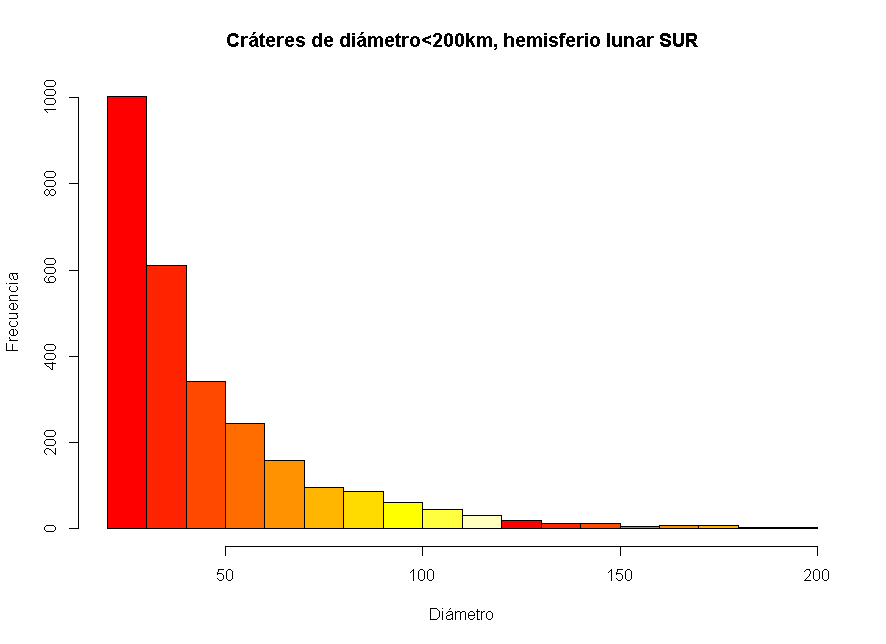
\includegraphics[width=12cm]{../fig/cap09-cratereslunares.png}
\end{enColor}
\begin{bn}
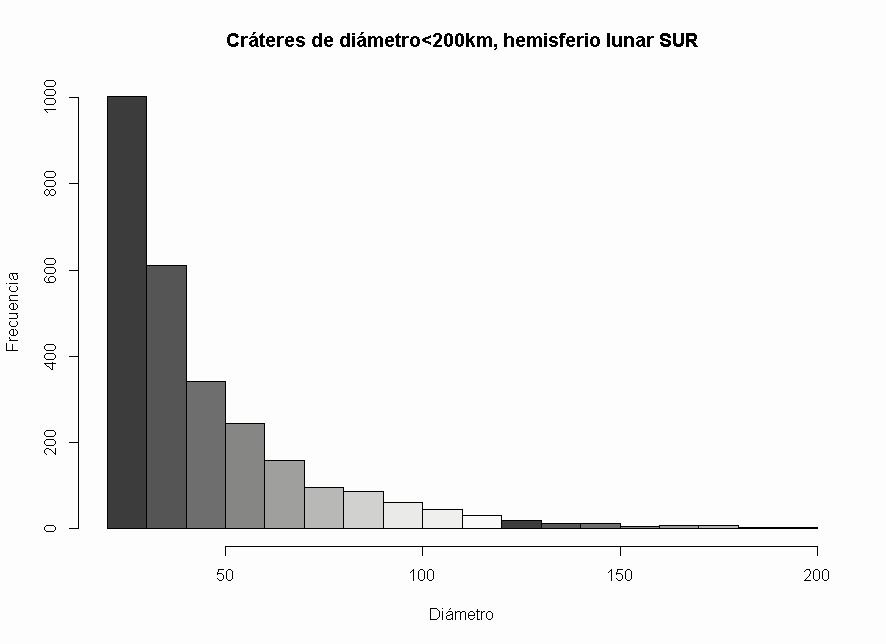
\includegraphics[width=12cm]{../fig/cap09-cratereslunares-bn.png}
\end{bn}
\caption{Distribución de diámetros ($<200$ km), de cráteres del hemisferio sur lunar}
\label{cap09:fig:CrateresLuna}
\end{center}
\end{figure}

Esta figura, que evidentemente no se corresponde a una distribución normal, debería hacer que te
replantearas lo que hemos hecho en este ejemplo. Daremos más detalles en el Apéndice
\ref{apendice:MasAlla}. \qed
\end{ejemplo}

\subsection{Intervalos de confianza vs contrastes.}
\label{cap09:subsec:IntervalosDeConfianzaVsContrastes01}

Vamos a dedicar este apartado a discutir un aspecto de la relación entre contrastes de hipótesis e intervalos de confianza que, a menudo, genera confusión, y que tradicionalmente no se aborda en muchos cursos de introducción a la Estadística.

Hemos visto que los intervalos de confianza nos permiten situar, con un cierto nivel de confianza,
la media de una población normal. Ahora, en un contraste como los de este capítulo, queremos saber
si las medias de dos poblaciones son o no iguales. La idea es demasiado tentadora: construimos dos
intervalos de confianza, uno para cada población, al nivel de confianza que se desee. Si esos dos
intervalos {\em no se solapan}, entonces las medias son significativamente distintas, al nivel de
confianza establecido. Veamos un ejemplo. \begin{ejemplo} \label{cap09:ejem:IntervalosVsContrastes}
El fichero
\begin{center}
\fichero{../datos/Cap09-IntervalosVsContrastesNoSolapan.csv}{Cap09-IntervalosVsContrastesNoSolapan.csv}
\end{center}
contiene dos muestras grandes (una en cada columna, con $n_1=n_2=100$) de dos poblaciones normales.
Se puede comprobar (y lo haremos en el Tutorial09) que los intervalos de confianza, al $95\%$ para
las medias de esas muestras son:
\[
\begin{cases}
\mbox{muestra1: }&133.4<\mu_1<135.6\\
\mbox{muestra2: }&138.4<\mu_2<141.2
\end{cases}
\]
y por lo tanto, esos intervalos no solapan. En la Figura
\ref{cap09:fig:IntervalosDeConfianzaVsContrastes01} se muestran esos intervalos de confianza.

\begin{figure}[ht]
\begin{center}
\begin{enColor}
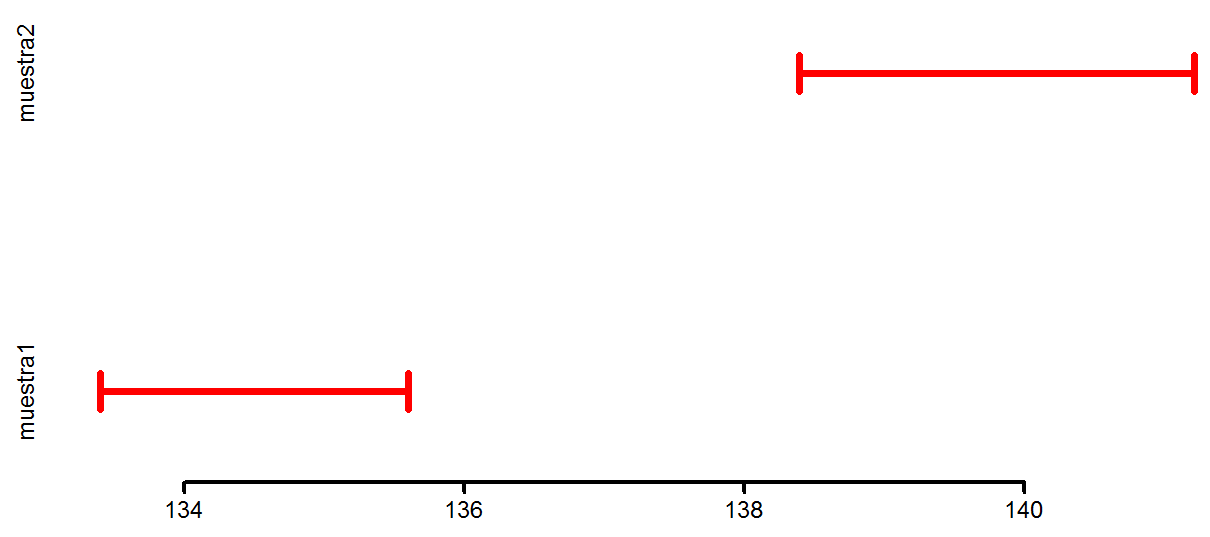
\includegraphics[width=9cm]{../fig/Cap09-IntervalosVsContrastes01.png}
\end{enColor}
\begin{bn}
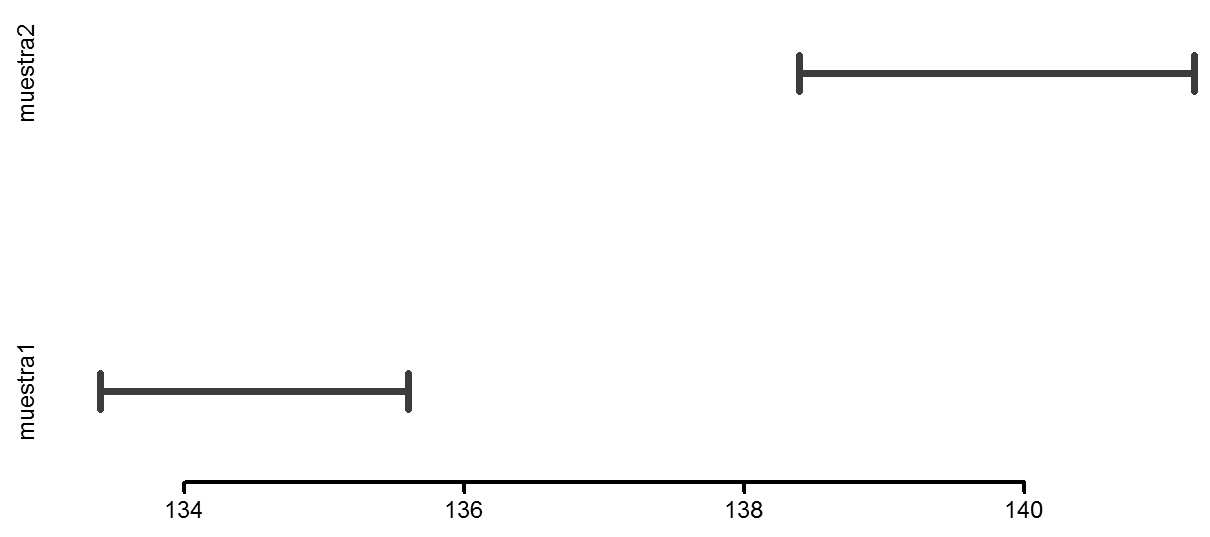
\includegraphics[width=9cm]{../fig/Cap09-IntervalosVsContrastes01-bn.png}
\end{bn}
\caption{Intervalos de confianza para el primer caso del Ejemplo \ref{cap09:subsec:IntervalosDeConfianzaVsContrastes01}}
\label{cap09:fig:IntervalosDeConfianzaVsContrastes01}
\end{center}
\end{figure}
Si realizamos un contraste de diferencia de medias, usando los métodos del caso (b) de la Sección
\ref{cap09:sec:diferenciaMediasDosPoblaciones} (pág.
\pageref{cap09:sec:diferenciaMediasDosPoblaciones}), obtenemos un p-valor aproximadamente igual a
$6.22\cdot 10^{-9}$. Es decir, que podemos concluir que las medias son significativamente
diferentes, como parece indicar la Figura \ref{cap09:fig:IntervalosDeConfianzaVsContrastes01}.

Por otra parte, el fichero \begin{center}
\fichero{../datos/Cap09-IntervalosVsContrastesSolapan.csv}{Cap09-IntervalosVsContrastesSolapan.csv}
\end{center}
contiene otras dos muestras de dos poblaciones normales (de nuevo, con $100$ elementos en cada muestra). Las medias son las mismas que en el primer caso, pero hemos aumentado la desviación típica de las poblaciones. El resultado de ese aumento en la dispersión es que, ahora, los intervalos de confianza al $95\%$ para las medias son:
\[
\begin{cases}
\mbox{muestra1: }&131.4<\mu_1<137.6\\
\mbox{muestra2: }&136.4<\mu_2<143.2
\end{cases}
\]
y por lo tanto, en este caso los intervalos solapan, como muestra la Figura
\ref{cap09:fig:IntervalosDeConfianzaVsContrastes02}.
\begin{figure}[ht]
\begin{center}
\begin{enColor}
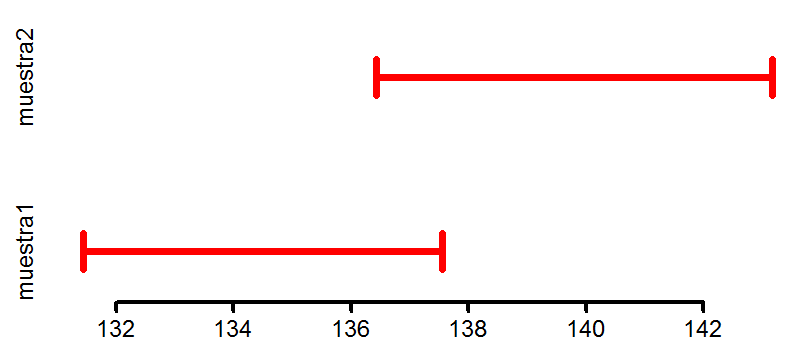
\includegraphics[width=9cm]{../fig/Cap09-IntervalosVsContrastes02.png}
\end{enColor}
\begin{bn}
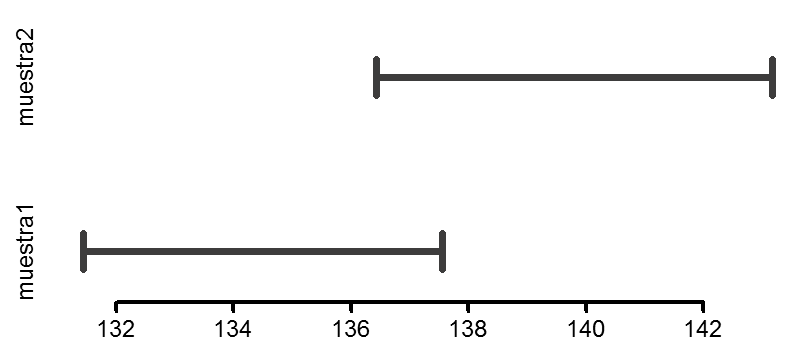
\includegraphics[width=9cm]{../fig/Cap09-IntervalosVsContrastes02-bn.png}
\end{bn}
\caption{Intervalos de confianza para el segundo caso del Ejemplo \ref{cap09:subsec:IntervalosDeConfianzaVsContrastes01}}
\label{cap09:fig:IntervalosDeConfianzaVsContrastes02}
\end{center}
\end{figure}
¿Cuál es la conclusión en este caso? Podemos decir, a la vista de esa figura, que rechazamos la hipótesis alternativa $H_a=\{\mu_1\neq \mu_2\}$ y decir que los datos no permiten concluir que las medias sean distintas (al $95\%$)?

Antes de concluir nada, hagamos también en este caso un contraste de diferencia de medias, usando otra vez  los métodos del caso (b) de la Sección \ref{cap09:sec:diferenciaMediasDosPoblaciones}. Se obtiene un p-valor aproximadamente igual a $0.02246$, que es $<0.05$, y que, desde luego, nos permitiría rechazar a un nivel de significación del $95\%$ la hipótesis nula $H_0=\{\mu_1=\mu_2\}$.

Está claro que no podemos rechazar ambas, $H_a$ y $H_0$. Y los métodos de la Sección \ref{cap09:sec:diferenciaMediasDosPoblaciones} son correctos, así que debe haber algo mal en esta forma de usar los intervalos de confianza para hacer contrastes de diferencia de medias.

El problema es, por decirlo de una manera sencilla, que los intervalos de confianza tratan a cada variable {\em por separado}. Y al hacerlo, sobrevaloran la probabilidad de que las dos medias se parezcan. Para ayudar al lector a ver esto, puede venir bien pensarlo de esta manera: para que, a partir de dos muestras de estas poblaciones, lleguemos a la conclusión de que las dos medias se parecen mucho, la media poblacional de la primera tiene que caer en la parte más alta de su intervalo de confianza (o más arriba aún), mientras que la media poblacional de la segunda población tiene que caer  en la parte baja de su intervalo de confianza (o más abajo aún). El contraste de diferencia de medias tiene esto en cuenta a la hora de calcular las probabilidades. Pero al fijarnos sólo en los intervalos de confianza, estamos asumiendo que esos dos sucesos, de por sí poco probables, ocurren simultáneamente. Y en eso radica nuestra sobreestimación de la probabilidad.
\qed
\end{ejemplo}

Como trata de poner de manifiesto este ejemplo, si se utilizan los intervalos de confianza, el contraste pierde {\em potencia} (en el sentido de la Sección \ref{cap07:sec:PotenciaContraste}, pág. \pageref{cap07:sec:PotenciaContraste}) , porque pierde capacidad de detectar que $H_0$ es falsa. Hemos argumentado que eso se debe a una sobreestimación de la probabilidad de que las medias se parezcan, pero podemos dar un argumento más formal. Si no lo entiendes al leerlo por primera vez, no te preocupes, lo importante es que retengas la idea que aparece destacada en la página \pageref{cap09:lugar:IntervalosVsContrastes}.

Cuando se usan los intervalos de confianza para el contraste, entonces el criterio es que rechazamos $H_a$ si los intervalos solapan. Recordemos que esos intervalos son:
\[
\begin{cases}
\mu_1=\bar X_1\pm z_{\alpha/2}\dfrac{s_1}{\sqrt{n_1}},&\mbox{ para la población $1$ y }\\[3mm]
\mu_2=\bar X_2\pm z_{\alpha/2}\dfrac{s_2}{\sqrt{n_2}},&\mbox{ para la población $2$.}
\end{cases}
\]
Para fijar ideas, vamos a suponer que $\bar X_2>\bar X_1$ (como en el Ejemplo \ref{cap09:ejem:IntervalosVsContrastes}). Entonces los intervalos solapan si el extremo inferior del intervalo para $\mu_2$ es más pequeño que el extremo superior del intervalo para $\mu_1$. Es decir, si se cumple:
\[ \bar X_2 - z_{\alpha/2}\dfrac{s_2}{\sqrt{n_2}} < \bar X_1 + z_{\alpha/2}\dfrac{s_1}{\sqrt{n_1}}\]
Y, despejando $z_{\alpha/2}$, esto se puede escribir:
\begin{equation}
\label{cap09:ecu:IntervalosVsContrastesMetodoIntervalos}
\dfrac{\bar X_2 - \bar X_1}{\dfrac{s_1}{\sqrt{n_1}} + \dfrac{s_2}{\sqrt{n_2}}} < z_{\alpha/2}
\end{equation}
Si se cumple esta desigualdad, entonces rechazamos $H_a=\{\mu_1\neq\mu_2\}$ (recuerda que suponemos $\bar X_2>\bar X_1$). Por contra, si usamos los métodos de la Sección \ref{cap09:sec:diferenciaMediasDosPoblaciones} , entonces el criterio para rechazar $H_a$ (cuando $\bar X_2>\bar X_1$) es que se cumpla la desigualdad:
\begin{equation}
\label{cap09:ecu:IntervalosVsContrastesMetodoContrastes}
    \dfrac{\bar X_2 - \bar X_1}{\sqrt{\dfrac{s_1^2}{n_1}+\dfrac{s_2^2}{n_2}}} < z_{\alpha/2}
\end{equation}
La diferencia entre ambos métodos está en el denominador. Para que sea más fácil compararlos, la Ecuación \ref{cap09:ecu:IntervalosVsContrastesMetodoIntervalos} se puede escribir:
\[\dfrac{\bar X_2 - \bar X_1}{\sqrt{\dfrac{s_1^2}{n_1}} + \sqrt{\dfrac{s_2^2}{n_2}}} < z_{\alpha/2}\]
Y ahora viene el hecho crucial. Sean cuales sean los números $n_1, n_2, s_1, s_2$, siempre se cumple que:
\begin{equation}
\label{cap09:ecu:IntervalosVsContrastesPitagoras}
\underbrace{
\dfrac{\bar X_2 - \bar X_1}{\sqrt{\dfrac{s_1^2}{n_1}} + \sqrt{\dfrac{s_2^2}{n_2}}}}
_{
\mbox{usando intervalos}
}
\leq
\underbrace{\dfrac{\bar X_2 - \bar X_1}{\sqrt{\dfrac{s_1^2}{n_1}+\dfrac{s_2^2}{n_2}}}}
_{
\mbox{método Sección \ref{cap09:sec:diferenciaMediasDosPoblaciones}}
}
\end{equation}

\noindent No queremos ponernos muy pesados con los detalles técnicos, pero con un cambio de variables, esto se reduce al teorema de Pitágoras de los triángulos rectángulos.

Hemos indicado a qué método corresponde cada fracción para ayudar a seguir la discusión. Porque, para nosotros, lo importante de la Ecuación \ref{cap09:ecu:IntervalosVsContrastesPitagoras} es que nos dice que si hemos rechazado $H_a$ usando los métodos de la Sección \ref{cap09:sec:diferenciaMediasDosPoblaciones}, entonces también la rechazaremos cuando usemos el método que consiste en ver si los intervalos de confianza solapan. Pero, y esta es la clave, {\em al revés no funciona}. Puede ocurrir que los intervalos solapen (el término izquierdo de la Ecuación \ref{cap09:ecu:IntervalosVsContrastesPitagoras} es menor que $z_{\alpha/2}$), pero que $H_a$ sea cierta.

    \begin{center}
    \fcolorbox{black}{Gris025}{
    \begin{minipage}{12.5cm}
        %%%%%%%%%%%%%%%%%%%%%%%%%%%%%%%%%%%%%%%
        {\centering
        \subsubsection*{Contraste de hipótesis vs intervalos de confianza.}
        \label{cap09:lugar:IntervalosVsContrastes}
        }
        %%%%%%%%%%%%%%%%%%%%%%%%%%%%%%%%%%%%%%%
         No es recomendable usar intervalos de confianza de cada  población, por separado, para contrastar la igualdad de medias en dos poblaciones. Si los intervalos al nivel de confianza $nc=1-\alpha$ no solapan, entonces las medias son significativamente distintas, al nivel de significación $ns=1-\alpha$. Pero {\bf si los intervalos de confianza solapan,
         no podemos usarlos para llegar a ninguna conclusión sobre el contraste de igualdad de
         medias}.
        %%%%%%%%%%%%%%%%%%%%%%%%%%%%%%%%%%%%%%%
    \end{minipage}}
    \end{center}
Queremos advertir al lector contra la práctica generalizada (y abusiva) de presentar, sobre todo en
forma gráfica, algún tipo de intervalo, más o menos directamente relacionado con los intervalos
de confianza de las medias,  sin acompañarlos de un contraste formal de diferencia de medias. Esta
situación resulta aún más grave por el hecho de que los intervalos que se representan, no son, a
menudo, intervalos de confianza, sino las llamadas {\sf barras de error estándar}\index{barras de
error estándar},  en inglés {\em SEM error bars}\index{error bars}\index{SEM error bars}, donde {\em SEM} es la
abreviatura de {\em Standard Error of the Mean}, o error estándar de la media, que ya apareció en el Teorema Central del Límite, y cuyo valor es:
\[SEM=\dfrac{s}{\sqrt{n}}.\]
Es decir, que con respecto al intervalo de confianza se ha eliminado el factor $z_{\alpha/2}$. La
Figura \ref{cap09:fig:GraficoBarrasError} muestra uno de esos (desafortunados) gráficos, cuyo uso
desaconsejamos.

\begin{figure}[ht]
\begin{center}
\begin{enColor}
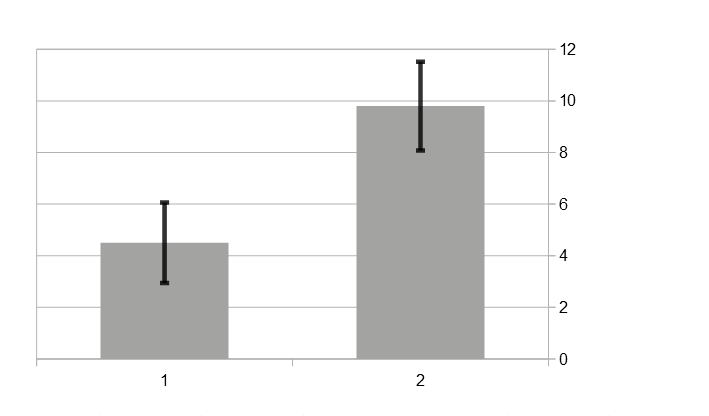
\includegraphics[width=9cm]{../fig/Cap09-GraficoConBarrasDeError-bn.png}
\end{enColor}
\begin{bn}
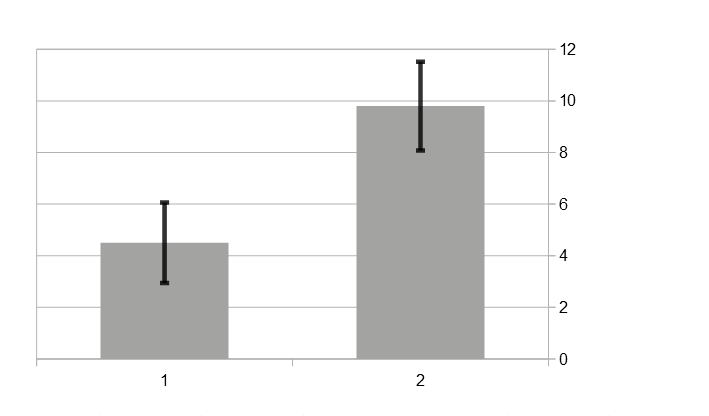
\includegraphics[width=9cm]{../fig/Cap09-GraficoConBarrasDeError-bn.png}
\end{bn}
\caption{Gráfico con barras de error estándar de la media.}
{\bf {!`}SE DESACONSEJA EL USO DE ESTE TIPO DE GRÁFICOS!}
\label{cap09:fig:GraficoBarrasError}
\end{center}
\end{figure}

Usar estos gráficos induce con frecuencia a errores en la interpretación de esos gráficos, cuando
se usan para hacer inferencia sobre las poblaciones. La confusión se debe a que, al usar las barras
de error las cosas son casi exactamente al revés que cuando se usan intervalos de confianza. En
poblaciones normales, unas barras de error estándar que solapan permiten rechazar $H_a$ (al
$95\%$), pero si las barras no solapan entonces no hay conclusiones evidentes. La razón técnica de
esto es la regla 68-95-99 de las poblaciones normales, junto con una desigualdad similar a la
Ecuación \ref{cap09:ecu:IntervalosVsContrastesPitagoras}, pero en sentido contrario. Concretamente,
sean cuales sean los valores de $n_1, n_2, s_1, s_2$, siempre se cumple que:
\begin{equation}
\label{cap09:ecu:IntervalosVsContrastesPitagorasAlReves}
\underbrace{\dfrac{\bar X_2 - \bar X_1}{\mathbf{\sqrt{2}}\cdot\sqrt{\dfrac{s_1^2}{n_1}+\dfrac{s_2^2}{n_2}}}}
_{
\mbox{método Sección \ref{cap09:sec:diferenciaMediasDosPoblaciones}}
}
\leq
\underbrace{
\dfrac{\bar X_2 - \bar X_1}{\sqrt{\dfrac{s_1^2}{n_1}} + \sqrt{\dfrac{s_2^2}{n_2}}}}
_{
\mbox{usando intervalos}
}
\end{equation}
{!`}Fíjate en la $\sqrt{2}$ del denominador de la izquierda!


Como se ve, el uso de las barras de error aumenta las posibilidades de una interpretación errónea
de los datos muestrales, especialmente cuando no se identifica con mucha claridad lo que
representan esas barras.


Volveremos a encontrarnos con este mismo problema en el Capítulo \ref{cap:IntroduccionAnova}, en el
que usaremos el llamado método Anova para contrastar la diferencia entre las medias de más de dos
poblaciones. Puedes leer una discusión más detallada sobre las barras de error, y los problemas que
plantean en el enlace [\,\ref{enlace0018}\,]\label{enlace0018a} (en inglés), o buscando en Internet páginas que contengan la expresión {\em dynamite plot}\index{dynamite plot}, que es como sus detractores suelen llamar a este tipo de gráficos.\\

\subsubsection{Intervalos de confianza unilaterales}

Vamos a aprovechar la discusión anterior para comentar otro aspecto de la relación entre contrastes e intervalos de confianza del que no nos hemos ocupado antes. Hemos comentado brevemente, en la página \pageref{cap07:lugar:ContrasteBilateralIntervaloConfianza}, que los contrastes de hipótesis bilaterales están relacionados con los intervalos de confianza, porque, en ese caso bilateral, los valores del parámetro que están fuera del intervalo de confianza (al nivel de confianza $nc=1-\alpha$), producen valores del estadístico situados en la región de rechazo (al nivel de significación $ns=1-\alpha$), y viceversa. Otra visión de esta misma idea ha aparecido al final de la Sección \ref{cap08:subsec:MetodoExactoBinomial}, cuando, al estudiar los intervalos de confianza exactos de Clopper-Pearson, hemos comentado que se podía {\em invertir} un contraste bilateral para obtener un intervalo de confianza.

En esos casos hablábamos siempre de contrastes bilaterales. Así que es natural preguntarse: ``¿hay algún análogo {\em unilateral} de los intervalos de confianza?'' La respuesta es  afirmativa:
    \begin{center}
    \fcolorbox{black}{Gris025}{
    \begin{minipage}{12.5cm}
        \begin{center}
        %%%%%%%%%%%%%%%%%%%%%%%%%%%%%%%%%%%%%%%
        {\bf  Intervalo de confianza unilateral.}\\
        \end{center}
       %%%%%%%%%%%%%%%%%%%%%%%%%%%%%%%%%%%%%%%
       Si $X$ es una variable aleatoria, un {\sf intervalo de confianza unilateral hacia la derecha}\index{intervalo de confianza unilateral}\index{unilateral, intervalo de confianza} (en inglés, {\em one-sided confidence interval}\index{confidence interval, one sided}) con una probabilidad $p$ dada, es un intervalo no acotado $(a,+\infty)$ tal que
       \begin{equation}\label{cap06:ecu:IntervaloConfianzaUnilateral}
           P(X>a)\geq p.
       \end{equation}
       Los intervalos de confianza unilaterales a la izquierda se definen de forma análoga.
       %%%%%%%%%%%%%%%%%%%%%%%%%%%%%%%%%%%%%%%
    \end{minipage}}
    \end{center}
Aunque la forma de construirlos (a partir del correspondiente estadístico) es bastante sencilla de imaginar, en el Tutorial09 veremos como obtener de forma sencilla algunos de estos intervalos de confianza unilaterales, usando el ordenador.

\subsection{El caso de datos emparejados.}
\label{cap09:subsec:CasoDatosEmparejados}

El problema que vamos a describir en esta sección se incluye en este capítulo porque el punto de partida son dos muestras, y a partir de ellas queremos calcular un contraste sobre diferencia de medias, usando la hipótesis de normalidad para la población. Hasta ahí, podrías pensar que estamos describiendo exactamente el mismo problema que acabamos de discutir. Pero hay un detalle esencial que cambia: aunque hay dos muestras no hemos dicho que haya dos poblaciones independientes. De hecho, cuando hablamos de un contraste de diferencia de medias con {\sf datos emparejados}\index{datos emparejados, contraste de diferencia de medias}\index{contraste de diferencia de medias para datos emparejados} (en inglés, {\em paired comparisons}\index{paired comparisons}), hablamos siempre de problemas en los que sólo hay una población. Un ejemplo típico, en el ámbito de la Medicina, es aquel en el que se mide una característica de un grupo de pacientes antes del tratamiento, y después del tratamiento se vuelve a medir esa misma característica en esos mismos pacientes, para ver si hay alguna diferencia (significativa) con los valores que se midieron antes. Veamos un ejemplo
\begin{ejemplo}
\label{cap09:ejem:DatosEmparejados01}
Para responder al desafío que supone la aparición en el mercado de {\em Pildorín Complex} (ver Ejemplo \ref{cap07:ejem:CangurosDepresivos01}, pág. \pageref{cap07:ejem:CangurosDepresivos01}), el laboratorio de la competencia ha desarrollado una nueva formulación de su tratamiento {\em Saltaplus Forte}, y quiere determinar si esta nueva versión es eficaz. Para ello, se ha medido la altura de los saltos de diez canguros depresivos elegidos al azar, antes y después del tratamiento con el nuevo {\em Saltaplus}. Los valores medidos (en metros) se muestran en la Tabla \ref{cap09:tabla:EjemploContrasteDatosEmparejados01}.

\begin{table}[htb]
{\small
    \begin{center}
    \begin{tabular}{|l|r|r|r|r|r|r|r|r|r|r|}
    \hline
    Paciente número:&1&2& 3 & 4 & 5 & 6 & 7 & 8 & 9 & 10 \\
    \hline
    Altura antes& 1.80 & 2.48 & 2.33 & 3.28 & 1.24 & 2.49 & 2.44 & 2.54 & 2.59 & 3.90\\
    \hline
    Altura después & 3.31 & 2.33 & 2.65 & 2.16 & 1.62 & 3.15 & 2.14 & 4.01 & 2.42 & 2.91  \\
    \hline
    \end{tabular}
    \end{center}
}
\caption{Tabla de valores medidos para el Ejemplo \ref{cap09:ejem:DatosEmparejados01}}
\label{cap09:tabla:EjemploContrasteDatosEmparejados01}
\end{table}
\noindent Las dos filas de esa tabla no pueden considerarse, en modo alguno, como muestras independientes. Los dos valores de cada una de las columnas se refieren a un individuo concreto, a un canguro en particular, el mismo en los dos casos.
\qed
\end{ejemplo}
En un contraste de datos emparejados tenemos dos muestras, ambas de tamaño $n$, que llamaremos $a$ y $b$, que desde luego no son independientes, y además tenemos un cierto emparejamiento dos a dos de los valores de la variable $X$ en ambas muestras, como se refleja en la Tabla \ref{cap09:tabla:ContrasteDatosEmparejados}, que es la versión general de la Tabla \ref{cap09:tabla:EjemploContrasteDatosEmparejados01} del Ejemplo \ref{cap09:ejem:DatosEmparejados01}.

\begin{table}[htb]
    \begin{center}
    \begin{tabular}{|l|c|c|c|c|}
    \hline
    Valor individual:&1&2&$\cdots$ &n\\
    \hline
    Muestra $a$&$x_{a, 1}$&$x_{a, 2}$&$\cdots$&$x_{a, n}$\\
    \hline
    Muestra $b$&$x_{b, 1}$&$x_{b, 2}$&$\cdots$&$x_{b, n}$\\
    \hline
    \end{tabular}
    \end{center}
\caption{Tabla de valores muestrales para un contraste de datos emparejados}
\label{cap09:tabla:ContrasteDatosEmparejados}
\end{table}

En este caso, insistimos, no se puede considerar las dos filas de la Tabla
\ref{cap09:tabla:ContrasteDatosEmparejados} como si fueran muestras de poblaciones independientes.
Lo que nos interesa es la {\em diferencia} entre los valores emparejados de esas muestras. Así
pues, la variable de interés para el contraste es $Y=X_b-X_a$, cuyos valores son las diferencias:
\[
y_1=(x_{b, 1}-x_{a, 1}), y_2=(x_{b, 2}-x_{a, 2}), \ldots, y_n=(x_{b, n}-x_{a, n}).
\]
Al considerar esas diferencias, el problema se reduce a un contraste de hipótesis para una única
población normal (la que representa la variable $Y$), y se aplican los métodos que vimos en el
Capítulo \ref{cap:ContrasteHipotesis}. Por supuesto, la hipótesis que se contrasta para la variable
$Y$ depende de cuál fuera nuestra intención al contrastar la diferencia de medias entre las
muestras $a$ y $b$.  En un ejemplo médico en el que queremos demostrar que el tratamiento ha
disminuido la media de cierta cantidad medida en los pacientes, si $a$ es la muestra {\em antes}
del tratamiento, y $b$ es la muestra post-tratamiento, entonces el contraste natural usará la
hipótesis alternativa
\[H_a=\{\mu_Y < 0\},\]
porque ese valor negativo de $\mu_Y$ es el que indica precisamente una disminución en los valores de $X$ medidos en los pacientes antes después del tratamiento, comparados con los valores medidos antes de aplicarlo.  En el lenguaje del Capítulo \ref{cap:ContrasteHipotesis}, estaríamos usando $\mu_0=0$ para la variable $Y$.

Si, por el contrario, queremos demostrar que ha habido un aumento de la media tras el tratamiento, usaremos:
\[H_a=\{\mu_Y > 0\},\]
\begin{ejemplo}
{\bf (Continuación del Ejemplo \ref{cap09:ejem:DatosEmparejados01})}
\label{cap09:ejem:DatosEmparejados02}
Los valores de la variable diferencia para este ejemplo aparecen en la última fila de la Tabla \ref{cap09:tabla:EjemploContrasteDatosEmparejados02}.
\begin{table}[htb]
{\scriptsize
    \begin{center}
    \begin{tabular}{|l|r|r|r|r|r|r|r|r|r|r|}
    \hline
    Paciente número:&1&2& 3 & 4 & 5 & 6 & 7 & 8 & 9 & 10 \\
    \hline
    Altura antes& 1.80 & 2.48 & 2.33 & 3.28 & 1.24 & 2.49 & 2.44 & 2.54 & 2.59 & 3.90\\
    \hline
    Altura después & 3.31 & 2.33 & 2.65 & 2.16 & 1.62 & 3.15 & 2.14 & 4.01 & 2.42 & 2.91  \\
    \hline
    Y= después - antes & 1.51& -0.15& 0.32& -1.12& 0.38& 0.66& -0.30& 1.47& -0.17& -0.99  \\
    \hline
    \end{tabular}
    \end{center}
}
\caption{Variable diferencia $Y=\mbox{después}-\mbox{antes}$ para el Ejemplo \ref{cap09:ejem:DatosEmparejados01}}
\label{cap09:tabla:EjemploContrasteDatosEmparejados02}
\end{table}

\noindent
En este ejemplo (ten en cuenta que  $\bar X_{\mbox{\tiny antes}}=2.51$ y $\bar X_{\mbox{\tiny después}}=2.67$) la hipótesis alternativa se puede expresar así:
\[H_a=\{\mu_{\mbox{\tiny después}}>\mu_{\mbox{\tiny antes}}\}\]
o, en términos de $Y$
\[H_a=\{\mu_Y > 0\},\]
Además, los valores muestrales son $n=10$, $\bar Y=\bar X_{\mbox{\tiny después}}-\bar X_{\mbox{\tiny antes}}=0.16$, $s_Y=0.896$. Calculamos el estadístico adecuado, que es (recuerda que usamos $\mu_0=0$):
\[\dfrac{\bar Y-\mu_0}{\dfrac{s_Y}{\sqrt{n}}}=\dfrac{0.16}{\dfrac{0.896}{\sqrt{10}}}\approx 0.56764\]
Y ahora, teniendo presente la forma de la hipótesis alternativa, calculamos el p-valor usando la cola derecha de la distribución $t$ de Student adecuada (con $9$ grados de libertad):
\[
p-valor=P(T_9>0.56764)\approx 0.2921
\]
Evidentemente, con este p-valor no rechazamos la hipótesis nula, así que la conclusión es que no hay evidencia empírica para afirmar que la altura media de los saltos haya aumentado con el tratamiento. El nuevo {\em Saltaplus} no parece dar resultados significativos.
\qed
\end{ejemplo}
Como puede verse, al expresarlo en términos de la  variable $Y$, el problema se reduce a un problema típico del Capítulo \ref{cap:ContrasteHipotesis}. Su presencia en este capítulo, aparte del hecho más o menos anecdótico de que partimos de dos muestras, sirve de recordatorio de que, al hacer un contraste de diferencia de medias como los de los apartados anteriores (no emparejados), {\em  debemos siempre comprobar que las muestras son realmente independientes}.

Aunque, como hemos dicho, este caso se reduce a un contraste como los que hemos aprendido a hacer en el Capítulo \ref{cap:ContrasteHipotesis}, y en el Tutorial07, veremos,  en el Tutorial09, una manera abreviada de hacer este tipo de contrastes a partir de las dos muestras iniciales, sin necesidad de construir explícitamente la variable diferencia $Y$. Y un último comentario: en el Ejemplo \ref{cap09:ejem:DatosEmparejados02} hemos usado la distribución $T$ para el contraste porque la muestra (las muestras emparejadas, hablando con propiedad) eran de tamaño pequeño ($n=10$). Si tuviéramos que hacer un contraste de datos emparejados con muestras emparejadas grandes, podríamos usar la normal estándar $Z$ para el contraste, como en el Capítulo \ref{cap:ContrasteHipotesis}.

\section{Cociente de varianzas en dos poblaciones normales. Distribución $F$ de Fisher-Snedecor.}
\label{cap09:sec:CocienteVarianzas2PoblacionesDistribucionF}

Aparte del interés que, por si mismo, pueda tener el problema de saber si las varianzas de dos poblaciones son iguales, hemos visto en la sección anterior que, para hacer inferencia sobre la diferencia de medias entre dos poblaciones normales independientes, a veces es necesario saber si las varianzas de ambas poblaciones son iguales (aunque desconozcamos los valores de esas varianzas).

Necesitamos por lo tanto pensar en algún tipo de pregunta, que nos permita saber si los dos números $\sigma_1^2$ y $\sigma_2^2$ son, o no, iguales. A poco que se piense sobre ello, hay dos candidatos naturales:
\begin{enumerate}
    \item Podemos estudiar la diferencia $\sigma_1^2-\sigma_2^2$ y ver si está cerca de $0$.
    \item O podemos estudiar el cociente $\dfrac{\sigma_1^2}{\sigma_2^2}$ y ver si está cerca de $1$.
\end{enumerate}
¿Cuál de los dos es el más adecuado? Es conveniente pensar sobre un ejemplo. Supongamos que $\sigma_1^2=\dfrac{1}{1000}$, $\sigma_2^2=\dfrac{1}{1000000}$. Entonces
    \[\sigma_1^2-\sigma_2^2=0.000999,\quad\mbox{mientras que }\quad\dfrac{\sigma_1^2}{\sigma_2^2}=1000.\]
A la vista de este ejemplo, la situación empieza a estar más clara. La diferencia  $\sigma_1^2-\sigma_2^2$ tiene el inconveniente de la {\em sensibilidad a la escala} en la comparación. Si empezamos con dos números {\em pequeños} (en las unidades del problema), entonces su diferencia es asimismo {\em pequeña} en esas unidades. Pero eso no impide que uno de los números sea órdenes de magnitud (miles de veces) más grande que el otro. En cambio, el cociente no tiene esta dificultad. Si el cociente de dos números es cercano a uno, podemos asegurar que los dos números son realmente parecidos, con independencia de la escala de medida. Por eso, a menudo, lo más adecuado es usar la {\em diferencia para comparar medidas de centralización} (medias, medianas, etc.), y en cambio usar el {\em cociente para comparar medidas de dispersión}, como varianzas, recorridos intercuartílicos, etc.

Por las razones expuestas, vamos a utilizar el cociente
    \[\dfrac{\sigma_1^2}{\sigma_2^2},\]
y trataremos de estimar si este cociente es un número cercano a uno. ¿Cómo podemos estimar ese cociente? Parece que el candidato natural para la estimación sería el cociente de las cuasivarianzas muestrales:
    \[\dfrac{s_1^2}{s_2^2}.\]
Y el siguiente paso para la inferencia es encontrar un estadístico que relacione este cociente con el cociente de varianzas, y cuya distribución muestral sea conocida. Para encontrar ese estadístico, recordemos (ver la Sección \ref{cap06:sec:InferenciaVarianzaDistribucionChi2}, y especialmente la Ecuación \ref{cap06:ecu:EstadisticoParaSigmaCuadrado}, pág. \pageref{cap06:ecu:EstadisticoParaSigmaCuadrado}) que, si $n_1$ y $n_2$ son los tamaños muestrales en ambas poblaciones, entonces
    \[k_1\dfrac{s_1^2}{\sigma_1^2}\sim\chi^2_{k_1},\quad\mbox{y análogamente }k_2\dfrac{s_2^2}{\sigma_2^2}\sim\chi^2_{k_2},\quad\mbox{ con }k_1=n_1-1,\quad k_2=n_2-1.\]
Y por lo tanto, dividiendo:
    \[\dfrac{s_1^2/s_2^2}{\sigma_1^2/\sigma_2^2}\sim\dfrac{\chi^2_{k_1}/k_1}{\chi^2_{k_2}/k_2}.\]
Esta relación estaría a un paso de lo que necesitamos para empezar la inferencia (intervalos y contrastes)...si supiéramos cómo se comporta el cociente de dos distribuciones de tipo $\chi^2$. Para describir estos cocientes, necesitamos introducir la última de las grandes distribuciones clásicas de la Estadística.

    \begin{center}
    \fcolorbox{black}{Gris025}{
    \begin{minipage}{12.5cm}
        \begin{center}
        %%%%%%%%%%%%%%%%%%%%%%%%%%%%%%%%%%%%%%%
        {\bf \sf Distribución $F$ de Fisher-Snedecor. }
        \index{distribución $F$ de Fisher-Snedecor}
        \end{center}
       %%%%%%%%%%%%%%%%%%%%%%%%%%%%%%%%%%%%%%%
        Una variable aleatoria $Y$ de la forma
        \[\dfrac{\chi^2_{k_1}/k_1}{\chi^2_{k_2}/k_2}\]
        es una variable de tipo Fisher-Snedecor $F_{k_1,k_2}$ con $k_1$ y $k_2$ grados de libertad. A veces escribimos  $F(k_1,k_2)$ si necesitamos una notación más clara.
       %%%%%%%%%%%%%%%%%%%%%%%%%%%%%%%%%%%%%%%
    \end{minipage}}
    \end{center}
Esta distribución recibe su nombre de los dos científicos que contribuyeron a establecer su uso en
Estadística, R. Fisher y G.W. Snedecor. De ellos, en particular, queremos destacar la figura de
Fisher, biólogo, genetista y a la vez el padre de la Estadística moderna. Puedes encontrar más
información sobre ambos usando el enlace [\,\ref{enlace0019}\,]\label{enlace0019a} de la Wikipedia (en inglés).

La función de densidad de $F_{k_1,k_2}$ es esta:
    \[f_{k_1,k_2}(x)=
        \begin{cases}
        \dfrac{1}{\beta\left(\dfrac{k_1}{2},\dfrac{k_2}{2}\right)}\left(\dfrac{k_1}{k_2}\right)^{k_1/2}\dfrac{x^{\frac{k_1}{2}-1}}{\left(1+\frac{k_1}{k_2}x\right)^{\frac{k_1+k_2}{2}}}&x\geq 0\\[6mm]
        0&x<0
        \end{cases}
    \]
donde $\beta$ es, de nuevo, la función beta, que ya apareció en relación con la $t$ de Student.
Como en casos anteriores, la incluimos por completitud, pero no vamos a necesitar su expresión para
nuestro trabajo. En cambio, si es importante que el lector se familiarice con el aspecto que
presentan las gráficas de estas funciones, para distintos valores de $k_1$ y $k_2$. La Figura
\ref{cap09:fig:DistribucionF} muestra el aspecto genérico de esta distribución. En el Tutorial09 veremos de forma dinámica como se modifica la distribución al cambiar $k_1$ y $k_2$.
%\begin{center}
%\fichero{../datos/Cap09-DistribucionF.html}{Cap09-DistribucionF.html}
%\end{center}
%permite experimentar de forma dinámica con distintos valores de $k_1, k_2$.
Hay dos aspectos de esta distribución que queremos destacar:
\begin{figure}[ht]
\begin{center}
\begin{enColor}
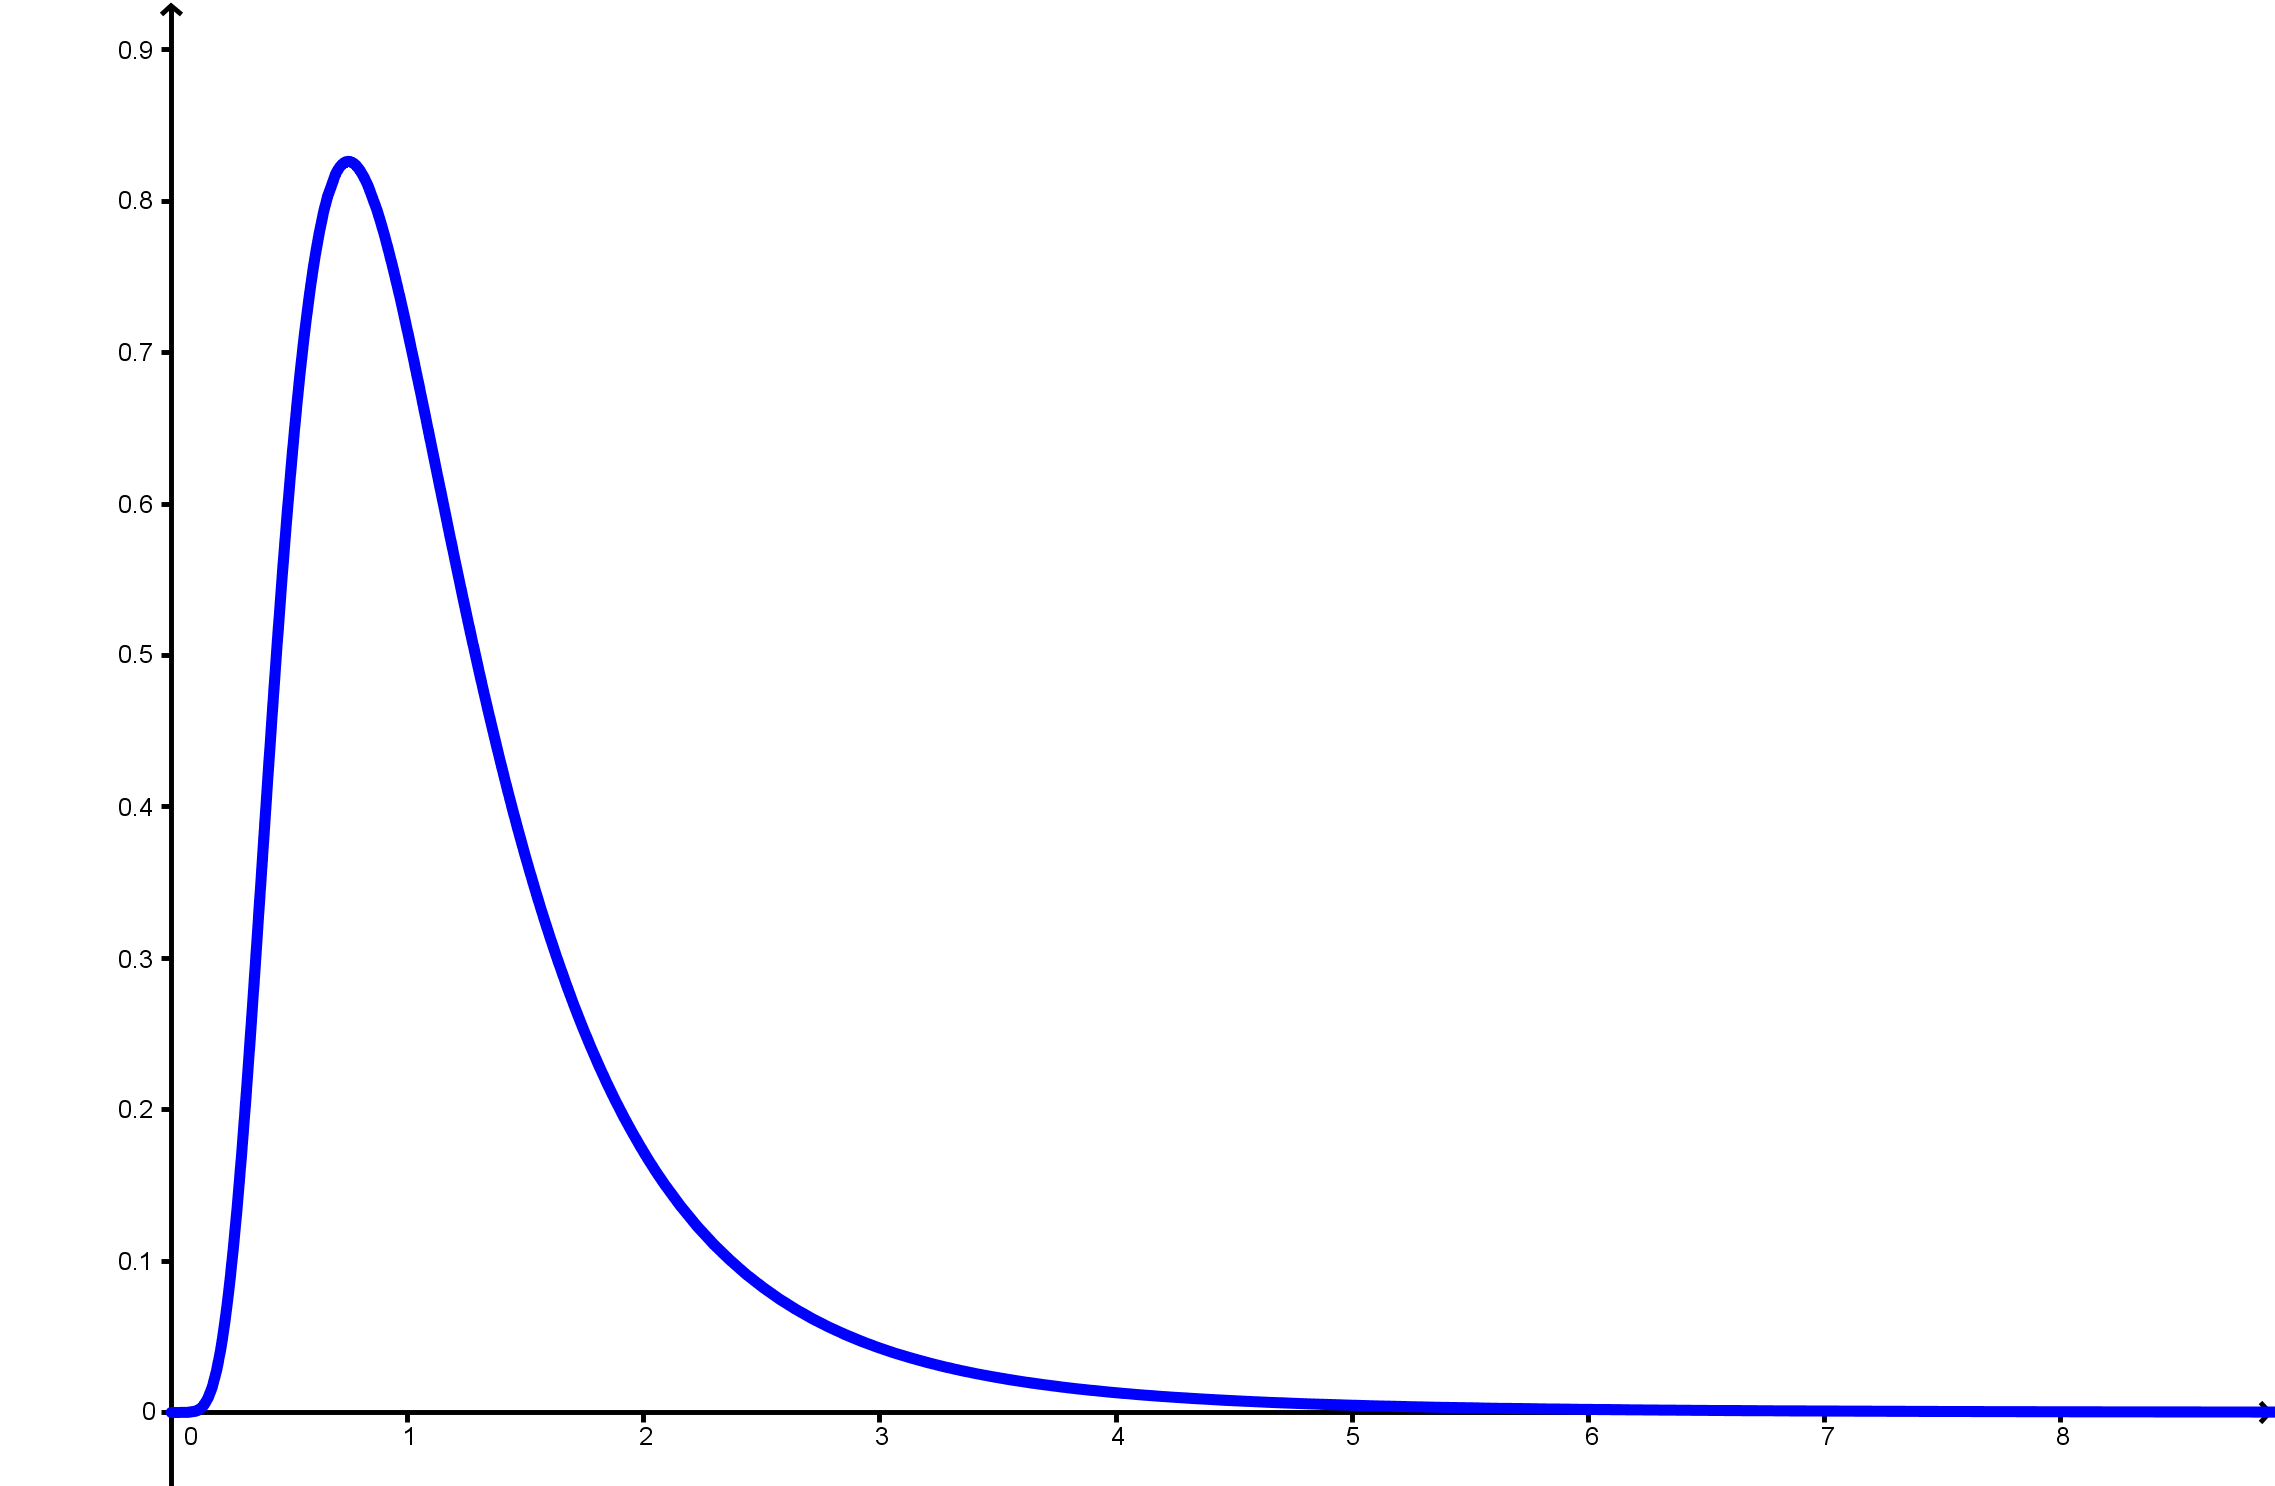
\includegraphics[width=12cm]{../fig/Cap09-DistribucionF.png}
\end{enColor}
\begin{bn}
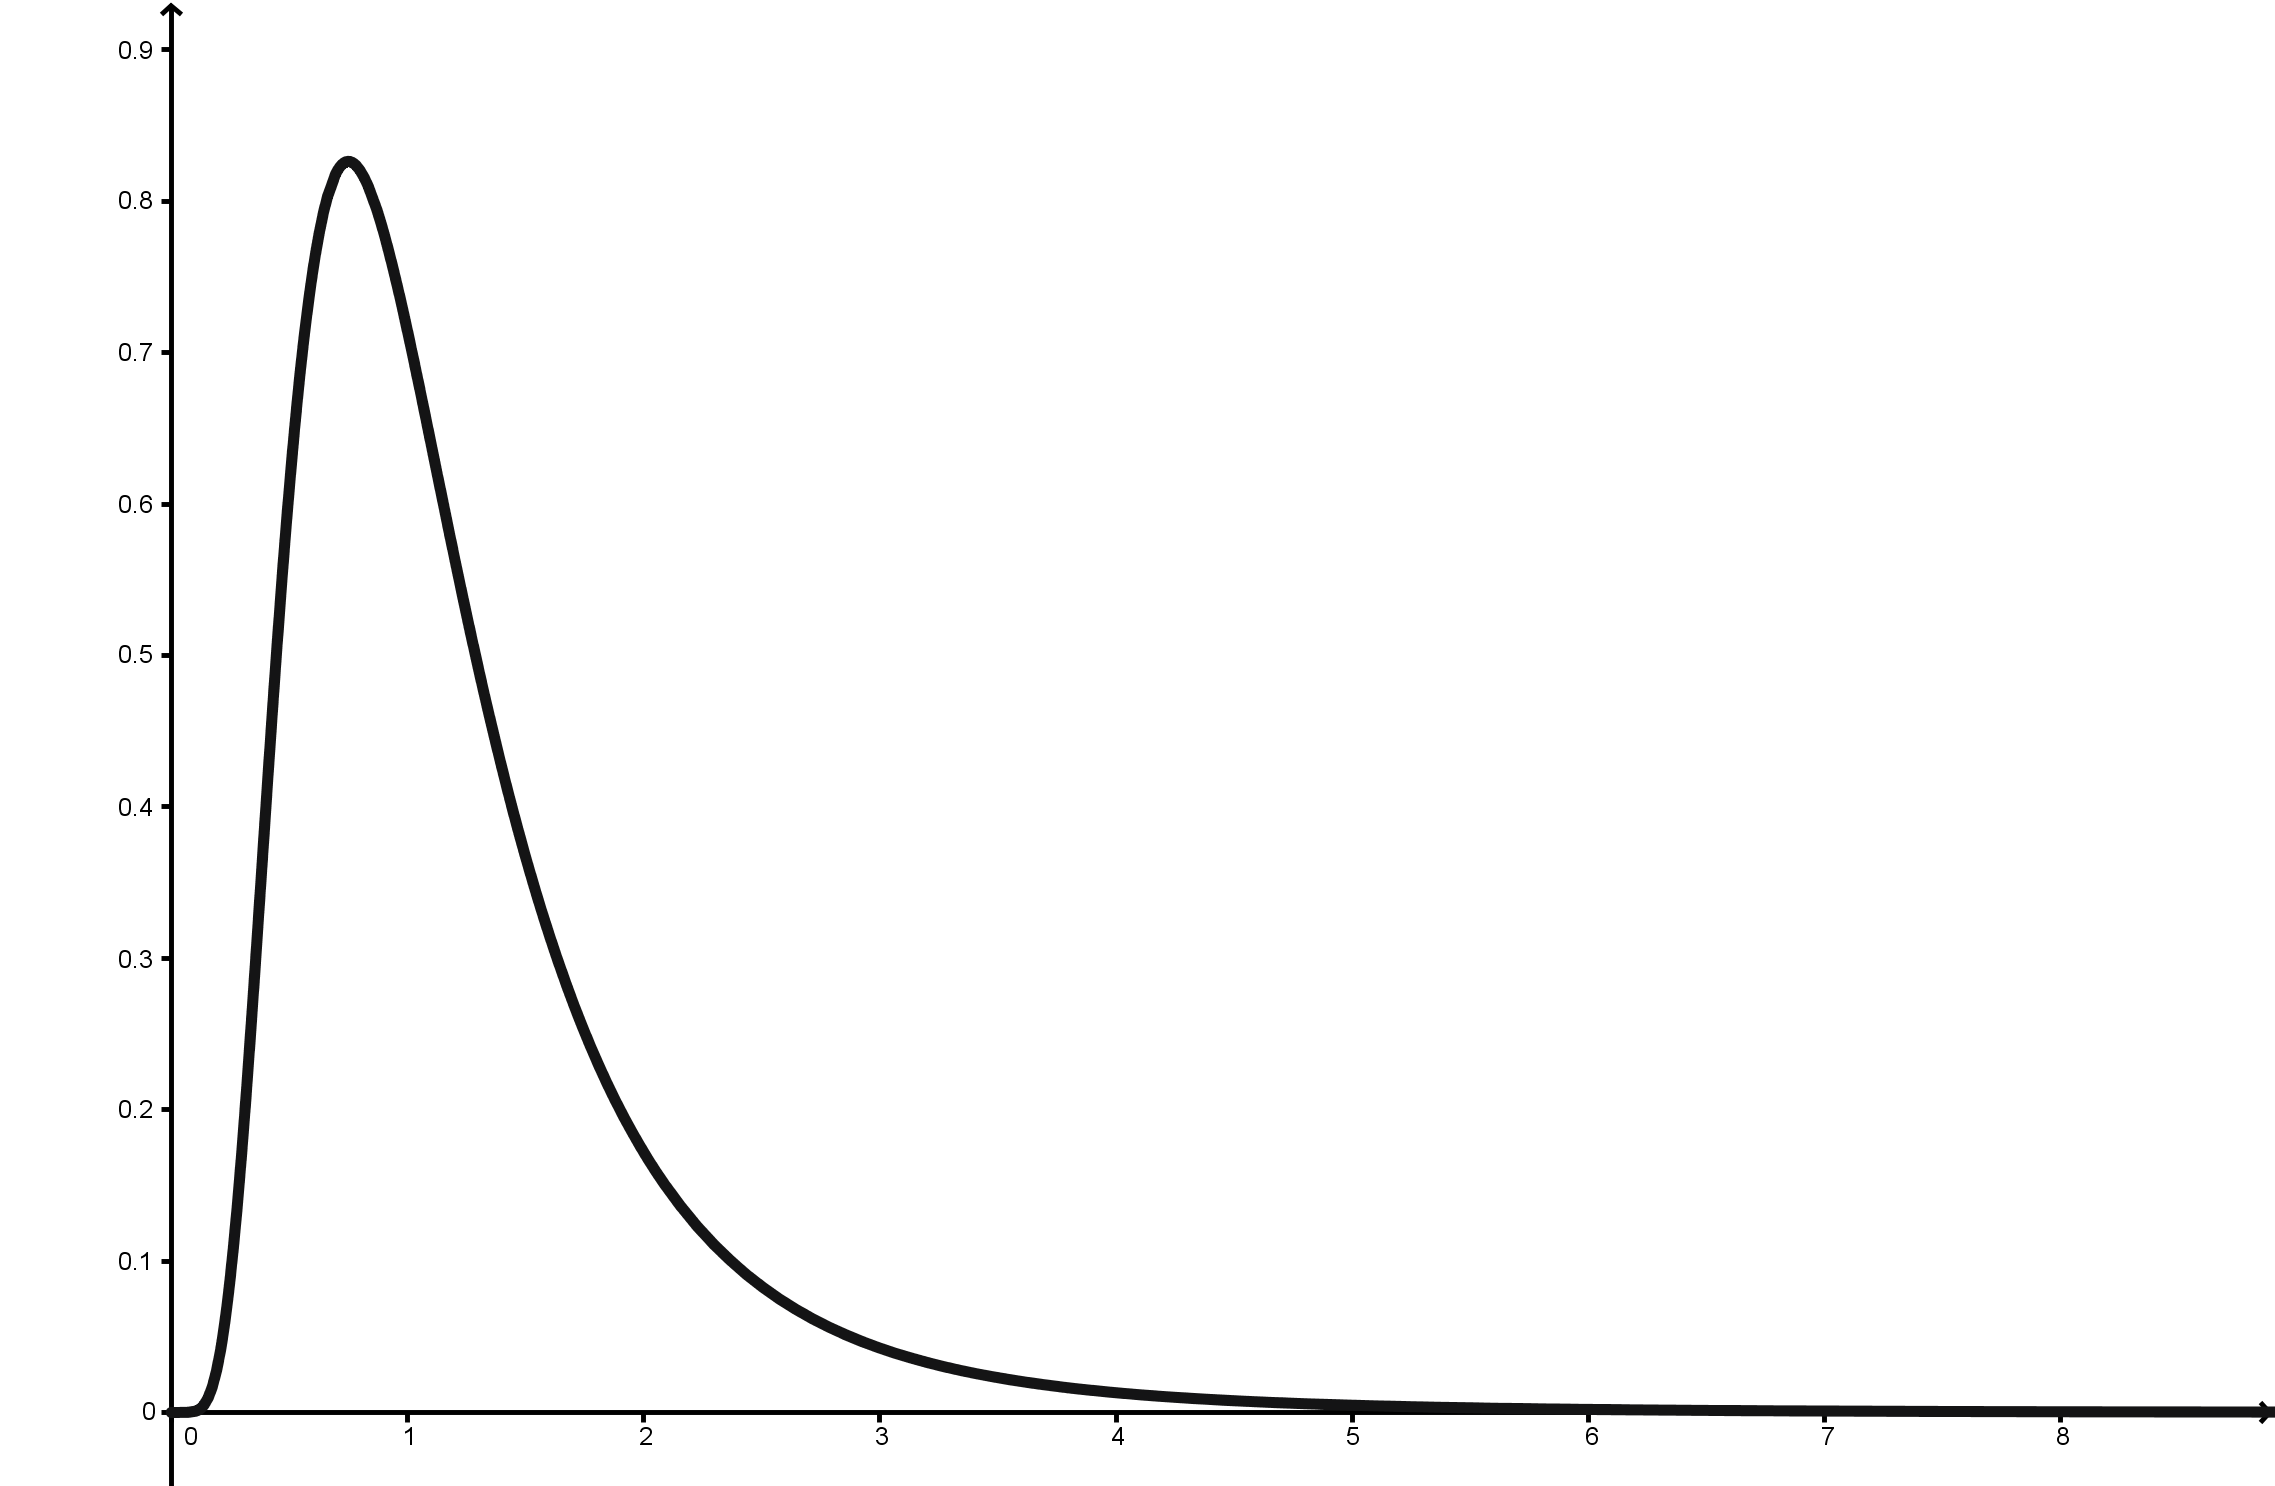
\includegraphics[width=12cm]{../fig/Cap09-DistribucionF-bn.png}
\end{bn}
\caption{Función de densidad de la distribución $F_{20,10}$}
\label{cap09:fig:DistribucionF}
\end{center}
\end{figure}

\begin{itemize}
  \item La función sólo toma valores no nulos en el semieje positivo.
  \item Y no es simétrica, como ocurría con la $\chi^2$.
\end{itemize}
La segunda de estas observaciones nos adelanta que tendremos que trabajar más cuando necesitemos los cuantiles de la distribución $F$. En relación con esto, en el Tutorial09 aprenderemos a resolver todos los problemas, directos e inversos, relacionados con la distribución de Fisher.

La notación que vamos a utilizar para los cuantiles de la distribución de Fisher es coherente con lo que venimos haciendo a lo largo del curso.
    \begin{center}
    \fcolorbox{black}{Gris025}{
    \begin{minipage}{12.5cm}
        \begin{center}
        %%%%%%%%%%%%%%%%%%%%%%%%%%%%%%%%%%%%%%%
        {\bf  Cuantiles de la distribución $F$.}\\
        \end{center}
        \index{distribución $F$, cuantiles.}\index{cuantiles de $F$}
        \index{$\chi^2$}
       %%%%%%%%%%%%%%%%%%%%%%%%%%%%%%%%%%%%%%%
       Si la variable aleatoria $Y$ tiene una distribución de tipo $F_{k_1,k_2}$, y $p_0$ es un valor cualquiera de probabilidad entonces $f_{k_1,k_2;p_0}$ es el valor que verifica:
       \begin{equation}\label{cap09:ecu:CuantilesF}
           P(F_{k_1,k_2}\geq f_{k_1,k_2;p_0})=p_0.
       \end{equation}
       es decir que deja probabilidad $p_0$ en su cola derecha, y $1-p_0$ en su cola izquierda.
       %%%%%%%%%%%%%%%%%%%%%%%%%%%%%%%%%%%%%%%
    \end{minipage}}
    \end{center}
Una observación: en algunos libros se utiliza (por ejemplo, para escribir los intervalos de confianza) esta propiedad de los cuantiles de la distribución $F$
    \[f_{k_1,k_2;p_0}=\dfrac{1}{f_{k_2,k_1;1-p_0}}.\]
Es decir, que podemos cambiar $\alpha$ por $1-\alpha$ si a la vez cambiamos $k_1$ por $k_2$ como en
la expresión anterior.
Esta propiedad permitía, entre otras cosas, disminuir el volumen de las tablas que se incluían en los libros. Pero, dado que nosotros vamos a calcular siempre esos valores usando el ordenador, no vamos a utilizarla.

Ahora que conocemos la distribución $F$, podemos usarla para volver a la inferencia sobre la diferencia de varianzas en el punto en el que la habíamos dejado. Ya tenemos el estadístico que se necesita:
\begin{center}
    \fcolorbox{black}{Gris025}{
    \begin{minipage}{12.5cm}
        %%%%%%%%%%%%%%%%%%%%%%%%%%%%%%%%%%%%%%%
        \begin{center}
        {\bf Estadístico para el cociente de varianzas.}
        \index{estadístico para el cociente de varianzas}
        \end{center}
       %%%%%%%%%%%%%%%%%%%%%%%%%%%%%%%%%%%%%%%
        Si las dos poblaciones son normales, entonces el estadístico:
        \begin{equation}\label{cap09:ecu:EstadisticoCocienteVarianzas}
        \Xi=\dfrac{s_1^2/s_2^2}{\sigma_1^2/\sigma_2^2}
        \end{equation}
        tiene una distribución de Fisher-Snedecor, de tipo $F_{k_1,k_2}$.
       %%%%%%%%%%%%%%%%%%%%%%%%%%%%%%%%%%%%%%%
    \end{minipage}}
\end{center}

\subsubsection{Intervalo de confianza para el cociente de varianzas}
\label{cap09:subsec:IntervaloConfianzaCocienteVarianzas}

Con esta información tenemos lo necesario para obtener el intervalo de confianza. Sin entreternos demasiado en los detalles, recordemos el esquema básico. Partimos de
\[P\left(f_{k_1,k_2;1-\alpha/2}< F_{k_1,k_2} <f_{k_1,k_2;\alpha/2}\right)=1-\alpha=nc\]
($nc$ es el nivel de confianza; piensa en $0.95$ para fijar ideas). Sustituimos aquí $F$ por el estadístico de la Ecuación \ref{cap09:ecu:EstadisticoCocienteVarianzas},
    \[P\left(f_{k_1,k_2;1-\alpha/2}< \dfrac{s_1^2/s_2^2}{\sigma_1^2/\sigma_2^2}< f_{k_1,k_2;\alpha/2}\right) =1-\alpha=nc,
    \]
y despejamos para dejar el cociente de varianzas en el centro de las desigualdades. El resultado que se obtiene es este:
\begin{center}
    \fcolorbox{black}{Gris025}{
    \begin{minipage}{12.5cm}
        %%%%%%%%%%%%%%%%%%%%%%%%%%%%%%%%%%%%%%%
        \begin{center}
        {\bf Intervalo de confianza para $\frac{\sigma_1^2}{\sigma_2^2}$, en dos poblaciones normales.}
        \index{intervalo de confianza para el cociente de varianzas}
        \index{cociente de varianzas, intervalo de confianza}
        \end{center}
       %%%%%%%%%%%%%%%%%%%%%%%%%%%%%%%%%%%%%%%
        Si las dos poblaciones son normales, y consideramos muestras independientes de tamaños $n_1$ y $n_2$ respectivamente, entonces el intervalo de confianza al nivel $nc=(1-\alpha)$  para el cociente de varianzas $\frac{\sigma_1^2}{\sigma_2^2}$  es:
            \begin{equation}\label{cap09:ecu:IntervaloConfianzaCocienteVarianzas}
            \dfrac{s_1^2}{s_2^2}\cdot\dfrac{1}{f_{k_1,k_2;\alpha/2}}\leq\frac{\sigma_1^2}{\sigma_2^2}\leq \dfrac{s_1^2}{s_2^2}\cdot\dfrac{1}{f_{k_1,k_2;1-\alpha/2}}.
            \end{equation}
        con $k_1=n_1-1$, $k_2=n_2-1$.
       %%%%%%%%%%%%%%%%%%%%%%%%%%%%%%%%%%%%%%%
    \end{minipage}}
\end{center}
Recomendamos al lector que relea los comentarios-advertencias que siguen a la Ecuación \ref{cap06:ecu:IntervaloConfianzaDesviacionTipica} (pág. \pageref{cap06:ecu:IntervaloConfianzaDesviacionTipica}), porque se aplican aquí, con las correcciones evidentes. En el Tutorial09 aprenderemos a usar el ordenador para automatizar estos cálculos.

%Veamos un ejemplo. \pendiente{(FALTA EJEMPLO)}

\subsubsection{Contraste de hipótesis para el cociente de varianzas}
\label{cap09:subsec:ContrasteHipotesisCocienteVarianzas}

El estadístico $\Xi$ de la Ecuación \ref{cap09:ecu:EstadisticoCocienteVarianzas} (pág. \pageref{cap09:ecu:EstadisticoCocienteVarianzas}) también nos permite obtener con sencillez los contrastes sobre el cociente de varianzas. Una observación: podríamos estar interesados en hacer contrastes con hipótesis alternativas del tipo
\[H_a=\left\{\frac{\sigma_1^2}{\sigma_2^2}> C_0\right\}\]
donde $C_0$ es cierta constante. Este tipo de contrastes son los adecuados cuando queremos saber si los datos respaldan la idea de que, por ejemplo, la varianza $s_1^2$ es al menos el doble de la varianza $s_2^2$. Aunque ese tipo de preguntas pueden tener su interés, lo cierto es que las preguntas que más a menudo nos vamos a hacer (con mucha diferencia), son las que tratan de averiguar si las dos varianzas son iguales, o si una es mayor que la otra (y que se corresponden con el caso $C_0=1$). Así que vamos a dar las fórmulas de los contrastes sólo para estos casos.

En particular, al utilizar  $C_0=1$ en todos estos casos, el estadístico $\Xi$ de la Ecuación \ref{cap09:ecu:EstadisticoCocienteVarianzas} (pág. \pageref{cap09:ecu:EstadisticoCocienteVarianzas}) se simplifica, de manera que, en lo que sigue, tenemos:
\[\Xi=\dfrac{s_1^2}{s_2^2}\]
que, como se ve, se calcula directamente a partir de las muestras. Con esto, los contrastes son:
\begin{enumerate}
    \item[(a)] Hipótesis nula: $H_0=\{\sigma_1^2\leq \sigma_2^2\}$.\\
     Región de rechazo: \[\dfrac{s_1^2}{s_2^2}>f_{k_1,k_2;\alpha}.\]\\
     p-valor=$P\left(F_{k_1,k_2}>\dfrac{s_1^2}{s_2^2}\right)$ (cola derecha)
    \item[(b)] Hipótesis nula: $H_0=\{\sigma_1^2\geq \sigma_2^2\}$.\\
     Región de rechazo: \[\dfrac{s_1^2}{s_2^2}<f_{k_1,k_2;1-\alpha}.\]\\
     p-valor=$P\left(F_{k_1,k_2}<\dfrac{s_1^2}{s_2^2}\right)$ (cola izquierda).
    \item[(c)] Hipótesis nula: $H_0=\{\sigma_1^2=\sigma_2^2\}$. Región de rechazo:
    \[\dfrac{s_1^2}{s_2^2}\mbox{ no pertenece al intervalo:}
        \left(f_{k_1,k_2;1-\alpha/2},f_{k_1,k_2;\alpha/2}\right).\]
        p-valor=$2\cdot P\left(F_{k_1,k_2}>\Xi\right)$ {!`}{!`}siempre que sea $\dfrac{s_1^2}{s_2^2}\geq 1$!! Si se tiene $\dfrac{s_1^2}{s_2^2}<1$, cambiar $s_1$ por $s_2$.
\end{enumerate}
Si la forma en la que hemos descrito la región de rechazo en el caso bilateral (c) te sorprende, recuerda que la hipótesis nula, en este caso, supone que $s_1^2/s_2^2=1$. Y ahora vuelve a mirar la Ecuación \ref{cap09:ecu:IntervaloConfianzaCocienteVarianzas} del intervalo de confianza en este caso.

\subsection{Ejemplos de contraste de diferencia de medias en muestras pequeñas de poblaciones normales.}
\label{cap09:subsec:EjemplosContrasteDiferenciaMediasUsandoT}

Estos contrastes nos permiten completar una tarea que habíamos dejado pendiente. Ahora podemos hacer contrastes de igualdad de medias en los casos (c) y (d) de la pág. \pageref{cap09:lugar:ContrasteDiferenciaMediasVarianzasIguales}, para lo cual,
previamente haremos un contraste de igualdad de varianzas.

%Veremos ejemplos de cada uno de esos dos tipos de contrastes en el Tutorial08.


\begin{ejemplo}
\label{cap09:ejem:ContrasteDiferenciaMediasVarianzasIguales}
Para cubrir el trayecto entre dos ciudades, se pueden utilizar dos medios de transporte público alternativos: el tren de cercanías y el autobús de línea. Se han medido los tiempos que empleaban en ese trayecto dos muestras independientes de $10$ viajeros cada una, en distintos días y horarios. Los viajeros de la primera muestra usaron el tren, mientras que los de la segunda muestra usaron el el autobús. Los tiempos (en minutos) que se han observado aparecen en la Tabla \ref{cap09:tabla:ejemploContrasteDiferneciaMediasVarianzasIguales}.
\begin{table}[ht]
\centering
\begin{tabular}{|l|rrrrrrrrrr|}
  \hline
  Tren $X_t$: & 94 & 95 & 93 & 96 & 96 & 90 & 95 & 94 & 97 & 92 \\
  \hline
  Bus $X_b$: & 100 & 97 & 99 & 98 & 100 & 100 & 94 & 97 & 95 & 97 \\
   \hline
\end{tabular}
\caption{Datos muestrales para el Ejemplo \ref{cap09:ejem:ContrasteDiferenciaMediasVarianzasIguales}}
\label{cap09:tabla:ejemploContrasteDiferneciaMediasVarianzasIguales}
\end{table}

Como hemos indicado en la tabla, $X_t$ es la variable ``duración (en minutos) del viaje en tren'', y $X_b$ la análoga para el autobús. A partir de esta tabla se obtienen estos valores muestrales (el subíndice $t$ se refiere a la muestra de viajeros del tren, y el subíndice $b$ a los del autobús):
\[
\begin{cases}
n_t=10,\quad \bar X_t=94.2,\quad s_t\approx 2.098\\[3mm]
n_b=10,\quad \bar X_b=97.7,\quad s_b\approx 2.111
\end{cases}
\]

¿Prueban estos datos que el  tren es más rápido que el autobús en ese trayecto? Para saberlo, vamos a  suponer que los tiempos de viaje por ambos medios siguen distribuciones normales, y llamemos $\mu_t$ a la duración media, en minutos, de los viajes en tren, mientras que $\mu_b$ es la duración media de los viajes en autobús. La hipótesis alternativa que queremos contrastar es, entonces:
\[H_a=\{\mu_t<\mu_b\}=\{\mu_t-\mu_b<0\}\]
Pero, para poder hacer ese contraste de diferencia de medias, primero necesitamos hacer una contraste de igualdad de varianzas, con hipótesis nula:
\[H_0=\{\sigma^2_t=\sigma^2_b\}\]
El estadístico adecuado para este contraste sobre las varianzas es
\[\dfrac{s_t^2}{s_b^2}=\left(\dfrac{2.098}{2.111}\right)^2\approx 0.9875\]
Con lo que el p-valor se calcula usando:
\[\mbox{p-valor}=2\cdot P\left(F_{9,9}>\dfrac{1}{0.9875}\right)\approx 0.9854\]
{!`}Fíjate en que hemos invertido el estadístico, al ser $s1<s2$! Con ese p-valor tan grande, no rechazamos la hipótesis nula. Eso significa que no tenemos razones para pensar que las varianzas sean distintas. Haremos, por tanto, un contraste de diferencia de medias suponiendo que las varianzas son iguales (el caso que hemos llamado (c) en la página \pageref{cap09:lugar:ContrasteDiferenciaMediasVarianzasIguales})
El estadístico adecuado, en este caso, es:
\[
    \sqrt{\left(\dfrac{(n_t-1)s_t^2+(n_b-1)s_b^2}{n_t+n_b-2}\right)
    \left(\dfrac{1}{n_t}+\dfrac{1}{n_b}\right)}\approx -3.719
\]
Y por lo tanto el p-valor es:
\[P(T_{18} < -3.719)\approx 0.0007848\]
con lo que, desde luego, rechazamos la hipótesis nula, para concluir que los datos apoyan la hipótesis de que en tren se tarda menos.
\qed
\end{ejemplo}
\noindent Veamos ahora un ejemplo del caso (d) de la página \pageref{cap09:lugar:ContrasteDiferenciaMediasVarianzasIguales}.
\begin{ejemplo}
\label{cap09:ejem:ContrasteDiferenciaMediasVarianzasDistintas}
Una asociación de consumidores tiene la sospecha de que la duración de las pausas publicitarias en una emisora de televisión aumentó, en el año 2013, en relación con el año anterior. La Tabla \ref{cap09:tabla:ejemploContrasteDiferneciaMediasVarianzasDistintas} contiene la duración, en minutos, de las pausas publicitarias, en sendas muestras aleatorias para cada uno de esos dos años.
\begin{table}[b]
\begin{center}
{\small
\begin{tabular}{|l|rrrrrrrrrrrr|}
  \hline
2012 & 1.87 & 2.14 & 1.69 & 2.32 & 2.36 & 1.10 & 2.11 & 2.00 & 2.52 & 1.46 & 1.94 & 1.46 \\
\hline
2013 & 2.37 & 2.30 & 2.65 & 2.46 & 2.01 & 2.22 & 2.12 & 2.25 & 2.40 & 2.44 & 2.44 & 2.47 \\
\hline
\end{tabular}
}
\end{center}
\caption{Datos de las muestras del Ejemplo \ref{cap09:ejem:ContrasteDiferenciaMediasVarianzasDistintas}}
\label{cap09:tabla:ejemploContrasteDiferneciaMediasVarianzasDistintas}
\end{table}
Usando el subíndice $2$ para los datos relativos al año $2012$, y el subíndice $3$ para los de $2013$, sean $X_2$ y $X_3$ las variables {``duración en minutos de la pausa publicitaria''} para los años 2012 y 2013, respectivamente. A partir de la Tabla \ref{cap09:tabla:ejemploContrasteDiferneciaMediasVarianzasDistintas} se obtienen estos valores muestrales:
\[
\begin{cases}
n_2=12,\quad \bar X_2=1.914,\quad s_2\approx 0.4216\\[3mm]
n_3=12,\quad \bar X_3=2.344,\quad s_3\approx 0.1740
\end{cases}
\]
Y la sospecha de la asociación de consumidores se concreta en la hipótesis alternativa:
\[H_a=\{\mu_2<\mu_3\},\]
siendo $\mu_2$ y $\mu_3$ las medias poblacionales de $X_2$ y $X_3$, respectivamente. Como en el anterior Ejemplo \ref{cap09:ejem:ContrasteDiferenciaMediasVarianzasIguales}, vamos a empezar por contrastar la hipótesis nula de igualdad de varianzas:
\[H_0=\{\sigma^2_2=\sigma^2_3\}\]
El estadístico de este contraste es
\[\dfrac{s_2^2}{s_3^2}=\left(\dfrac{0.4216}{0.1740}\right)^2\approx 5.871\]
Con lo que el p-valor se calcula usando:
\[\mbox{p-valor}=2\cdot P\left(F_{10,10}>5.871\right)\approx 0.006668\]
A la vista de este p-valor, rechazamos la hipótesis nula del contraste de igualdad de varianzas, y concluimos que hay razones para suponer que las varianzas $\sigma_2^2$ y $\sigma_3^2$ son distintas. Volviendo, con esta información, al contraste sobre la diferencia de medias, el estadístico adecuado para este caso (caso (d) de la página \pageref{cap09:lugar:ContrasteDiferenciaMediasVarianzasIguales}) es:
\[\Xi=\dfrac{\bar X_2-\bar X_3}{\scriptsize{\sqrt{\dfrac{s_2^2}{n_2}+\dfrac{s_3^2}{n_3}}}}
\approx -3.266\]
(Ver la Tabla \ref{tabla:EstadisticosContrastes} en el Apéndice \ref{apendice:Tablas}, \pageref{tabla:EstadisticosContrastes}). El número de grados de libertad, calculados con la aproximación de Welch (ver Ecuación \ref{ecu:aproximacionWelch}, pág. \pageref{ecu:aproximacionWelch}), es
\[k\approx 14.64\]
Como ya advertimos, se obtiene un número de grados de libertad fraccionario, pero eso no supone ninguna complicación adicional para el cálculo del p-valor, que es:
\[P(T_{k} < -3.266)\approx 0.001769\]
Puesto que el p-valor es muy pequeño, rechazamos la hipótesis nula del contraste de diferencia de medias, y concluimos que los datos respaldan las sospechas de la asociación de consumidores, y que la duración media de los anuncios ha aumentado.
\qed
\end{ejemplo}


\subsection{Contrastes y medida del tamaño del efecto.}
\label{cap09:subsec:MedidaTamannoEfecto}

Para cerrar esta sección, queremos volver brevemente, en el contexto de los contrastes sobre dos poblaciones de este capítulo, a la discusión de la página \pageref{cap07:subsubsec:AdvertenciaAbusoPValor}. Allí advertíamos contra un posible abuso de los p-valores, cuando se usan como el único criterio estadístico sobre el que basar una decisión. Para asegurarnos de que nuestros resultados son, además de estadísticamente significativos, científicamente relevantes, es necesario, como decíamos entonces, tener siempre en cuenta los tamaños de las muestras. Además, siempre hay que usar alguna forma de medida del {\em tamaño del efecto}. Hay muchas maneras de medir ese tamaño del efecto, que a su vez dependen del tipo de contraste (de medias o proporciones, en una o varias poblaciones, etc.). En un curso introductorio como este no podemos, ni queremos, entrar en detalle en esa discusión. Pero si queremos señalar, como principio general, que es {\em muy conveniente acompañar siempre los p-valores con un intervalo de confianza para la magnitud que se contrasta y de los correspondientes tamaños muestrales}.

Vamos a revisar algunos de los últimos ejemplos de este capítulo para ilustrar lo que decimos:
\begin{ejemplo}
Si, con los datos del Ejemplo \ref{cap09:ejem:ContrasteDiferenciaMediasVarianzasDistintas} calculamos un intervalo de confianza al $95\%$ para la diferencia de las medias $\mu_2-\mu_3$ (ver la Tabla \ref{tabla:IntervalosConfianzaDiferenciaMedias}(d), pág. \pageref{tabla:IntervalosConfianzaDiferenciaMedias}), se obtiene el intervalo:
\[(-0.7031, -0.1568)\]
Es decir, que la diferencia media en la duración de las pausas publicitarias que ha detectado el contraste, es (en valor absoluto) de entre $0.15$ y $0.7$ minutos, es decir, de entre unos 9 y unos 42 segundos. En cualquier caso, no llega a  un minuto. Como puede verse, la información que nos proporciona el intervalo de confianza complementa de manera muy adecuada al p-valor, y puede ser de suma importancia a la hora de decidir si estos datos son relevantes.

En el Ejemplo \ref{cap09:ejem:ContrasteDiferenciaMediasVarianzasIguales}, el del tren frente al autobús, se obtiene este intervalo de confianza al $95\%$ para la diferencia de medias $\mu_t-\mu_b$ (duración del viaje, en minutos):
\[(-5.48, -1.53)\]
Es decir, que la diferencia, a favor del tren, está entre un minuto y medio, y cerca de seis minutos. Presentada de esta forma, la información es seguramente más fácil de comprender y utilizar por los interesados.
\qed
\end{ejemplo}


\section{Riesgo relativo y el cociente de posibilidades (odds ratio).}
\label{cap09:sec:RiesgoRelativoCocienteProbabilidades}
\noindent{\bf Opcional: esta sección puede omitirse en una primera lectura.}\\

En esta sección vamos a volver sobre el problema con el que hemos abierto este capítulo, el del contraste para comparar las proporciones en dos poblaciones binomiales. ¿Por qué? Porque ahora hemos ganado la experiencia de otros tipos de contrastes, y porque el tema de esta sección se puede entender, al menos en parte, como una continuación de la discusión con la que comenzamos la Sección \ref{cap09:sec:CocienteVarianzas2PoblacionesDistribucionF} (pág. \pageref{cap09:sec:CocienteVarianzas2PoblacionesDistribucionF}). Allí, al hablar del contraste para comparar las varianzas de dos poblaciones normales, argumentábamos que, en ocasiones, era mejor utilizar el cociente, en lugar de la diferencia, para comparar dos cantidades. Y proponíamos, como recomendación genérica, usar la diferencia para las medidas de centralización (medias), y el cociente para las medidas de dispersión (varianzas).

Todo eso está muy bien, pero ¿qué ocurre cuando lo que se compara son proporciones? Una proporción es, en algunos sentidos, un objeto bastante parecido a una media; mira, por ejemplo la Ecuación \ref{cap08:ecu:ProporcionMuestral} (pág. \pageref{cap08:ecu:ProporcionMuestral}), que hemos usado para definir la proporción muestral. Y por eso, en la Sección \ref{cap09:subsec:ContrasteHipotesisDiferenciaProporciones} hemos considerado contrastes sobre la diferencia de proporciones, muy similares a los de las diferencias de medias.

Pero, por otra parte, una proporción está obligada a permanecer entre $0$ y $1$. Eso hace que, en ocasiones, en lugar de la diferencia entre dos proporciones, sea más relevante comparar sus tamaños relativos, y para eso es mejor usar el cociente. El siguiente ejemplo pretende servir de motivación para la discusión de esta sección.
\begin{ejemplo}
Supongamos que estamos estudiando dos poblaciones de la misma especie de microorganismos (por ejemplo, con medios de cultivo diferentes). Llamaremos $P_1$ y $P_2$ a esas poblaciones. Hemos observado, en una muestra de $1000$ individuos de la población $P_1$, que $9$ de ellos presentan una determinada mutación genética. En cambio, en una muestra de $800$ individuos de la población $P_2$, la mutación estaba presente en $4$ individuos. ¿Podemos afirmar que las proporciones de individuos con esa mutación son significativamente distintas en ambas poblaciones?

Las proporciones muestrales, de acuerdo con lo anterior, son:
    \[
    \begin{cases}
        \hat p_1=\dfrac{3}{1000}=0.009\\[3mm]
        \hat p_2=\dfrac{4}{800}=0.005
    \end{cases}
    \]
Así que la {\em diferencia} entre las proporciones muestrales es $\hat p_1-\hat p_2=0.004$. Una diferencia ¿realmente pequeña? Como otras veces en el curso, la pregunta es ¿comparado con qué? Si, por el contrario, comparamos las proporciones muestrales usando el cociente, tenemos:
\[\dfrac{\hat p_1}{\hat p_2}=\dfrac{0.009}{0.005}=1.8\]
Y esta información puede resultar mucho más relevante. Saber que la proporción es $1.8$ veces superior, es un dato que muchas veces marca el sentido de nuestras decisiones. ¿Cuál de estos dos titulares de periódico te parece más llamativo? ``Detectada una diferencia de $4$ milésimas en las proporciones'' o ``La proporción en la población $P_2$ es casi el doble que en la población $P_1$.''
\qed
\end{ejemplo}

Vamos a ponerle nombre a la cantidad que queremos analizar.
\begin{center}
    \fcolorbox{black}{Gris025}{
    \begin{minipage}{12.5cm}
        %%%%%%%%%%%%%%%%%%%%%%%%%%%%%%%%%%%%%%%
        \begin{center}
        {\bf Riesgo relativo (cociente de proporciones).}
        \index{riesgo relativo}\index{cociente de proporciones}
        \index{proporciones, cociente}\index{relative risk}\index{$RR$}
        \end{center}
       %%%%%%%%%%%%%%%%%%%%%%%%%%%%%%%%%%%%%%%
        Dadas dos poblaciones independientes, ambas de tipo Bernouilli, con proporciones de éxito iguales, respectivamente, a $p_1$ y $p_2$. Entonces el {\sf riesgo relativo} $RR$ (en inglés, {\em relative risk}) es el cociente:
        \begin{equation}
        \label{cap09:ecu:RiesgoRelativo}
        RR=\dfrac{p_1}{p_2}
        \end{equation}
       %%%%%%%%%%%%%%%%%%%%%%%%%%%%%%%%%%%%%%%
    \end{minipage}}
\end{center}

Naturalmente, el estimador natural del riesgo relativo es el cociente de proporciones muestrales, procedentes de sendas muestras independientes de ambas poblaciones:
    \begin{equation}
    \label{cap09:ecu:EstimadorMuestralRiesgoRelativo}
    \widehat{RR}=\dfrac{\hat p_1}{\hat p_2}
    \end{equation}
al que vamos a denominar {\sf riesgo relativo muestral}\index{riesgo relativo muestral}\index{$\widehat{RR}$}.
Para poder usar este estimador para hacer inferencia, necesitamos, como siempre, más información sobre su distribución muestral. Y aquí, por primera vez en el curso, surge la característica más importante de este problema. Vamos a utilizar una idea nueva, la de la {\sf transformación de variables}\index{transformación de variables}.  Veamos de qué se trata en un ejemplo.
\begin{ejemplo}
\label{cap09:ejem:TransformandoRiesgoRelativoConLogaritmos}
En algún sentido, este ejemplo está emparentado con el Ejemplo \ref{cap06:ejem:DistribucionMediaMuestral} (pág. \pageref{cap06:ejem:DistribucionMediaMuestral}), en el que explorábamos la distribución de la media muestral. Aquí nos proponemos estudiar cómo se distribuye el riesgo relativo muestral $\frac{\hat p_1}{\hat p_2}$, cuando consideramos muestras de dos poblaciones independientes. Naturalmente, vamos a fijarnos en un ejemplo concreto, y el lector puede preguntarse si el fenómeno que  vamos a observar se limita a este caso en particular. Después del ejemplo discutiremos eso con más detalle. Y en el Tutorial09 encontrarás el código que se ha usado para generar los datos de este ejemplo, y que puede modificarse fácilmente para explorar otros ejemplos.

Al trabajo. Tomamos dos poblaciones independientes en las que las proporciones poblacionales son iguales.
\[p_1=p_2=0.2.\]
Es decir, que en este caso sabemos de antemano que la hipótesis nula
\[H_0=\{p_1=p_2\},\mbox{ es decir }H_0=\left\{RR=\dfrac{p_1}{p_2}=1.\right\}\]
es cierta. Pero vamos a hacer como si no lo supiéramos, y vamos a tratar de usar el riesgo relativo muestral para contrastar esa hipótesis. Naturalmente, para hacer ese contraste, tomaríamos muestras de ambas poblaciones, y calcularíamos $\widehat{RR}$. Si la hipótesis nula es cierta (como, de hecho, sucede en este ejemplo), esperamos obtener, en la mayoría de las muestras, valores de $\widehat{RR}$ próximos a $1$.

Para comprobarlo, hemos programado en el ordenador una simulación en la que se generan $10000$ parejas de muestras, de tamaño $n=50$, de cada una de las poblaciones. En cada una de esas $10000$ parejas calculamos $\widehat{RR}$. El histograma de los $10000$ valores de $\widehat{RR}$ que hemos obtenido aparece en la parte (a) de la Figura \ref{cap06:fig:EjemploLogRR01}.

\begin{figure}[p]
\begin{center}
\begin{enColor}
(a)\\[3mm]
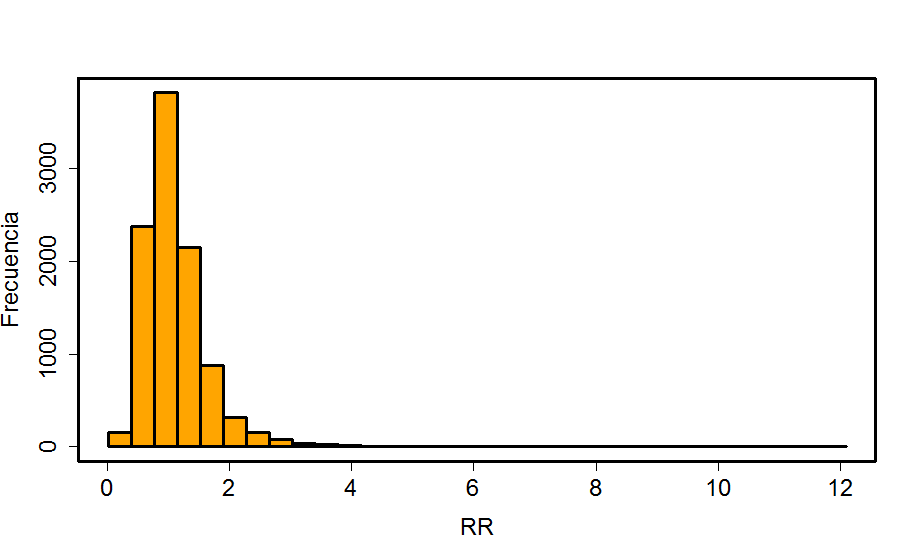
\includegraphics[width=13cm]{../fig/Cap09-EjemploLogRR01.png}\\[3mm]
(b)\\[3mm]
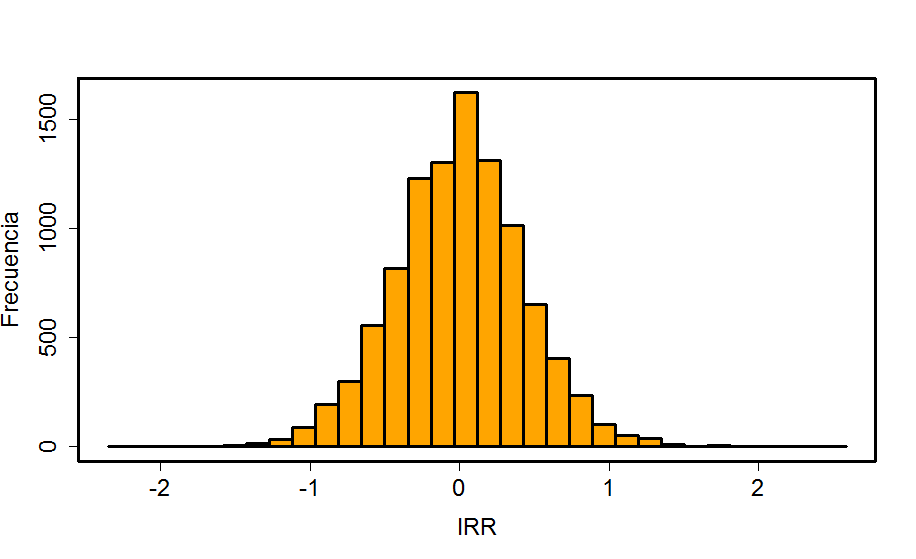
\includegraphics[width=13cm]{../fig/Cap09-EjemploLogRR02.png}
\end{enColor}
\begin{bn}
(a)\\[3mm]
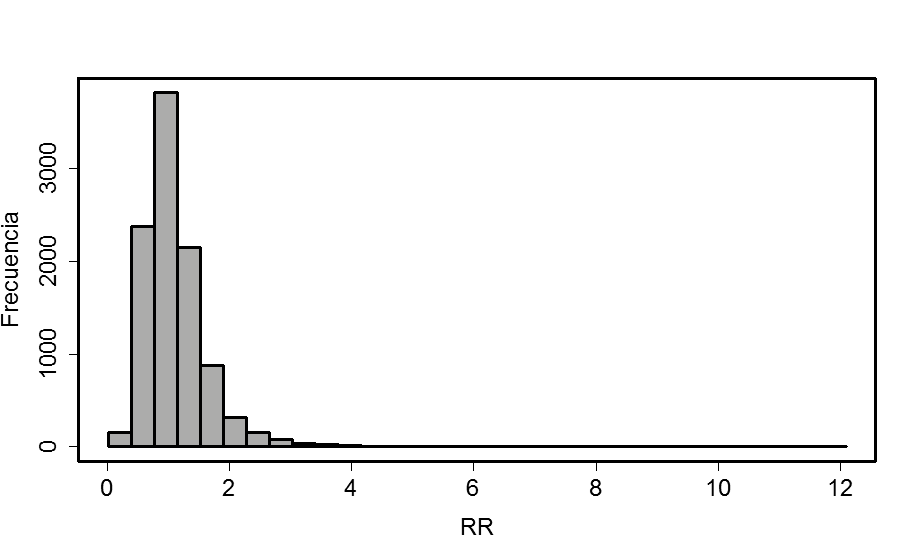
\includegraphics[width=13cm]{../fig/Cap09-EjemploLogRR01-bn.png}\\[3mm]
(b)\\[3mm]
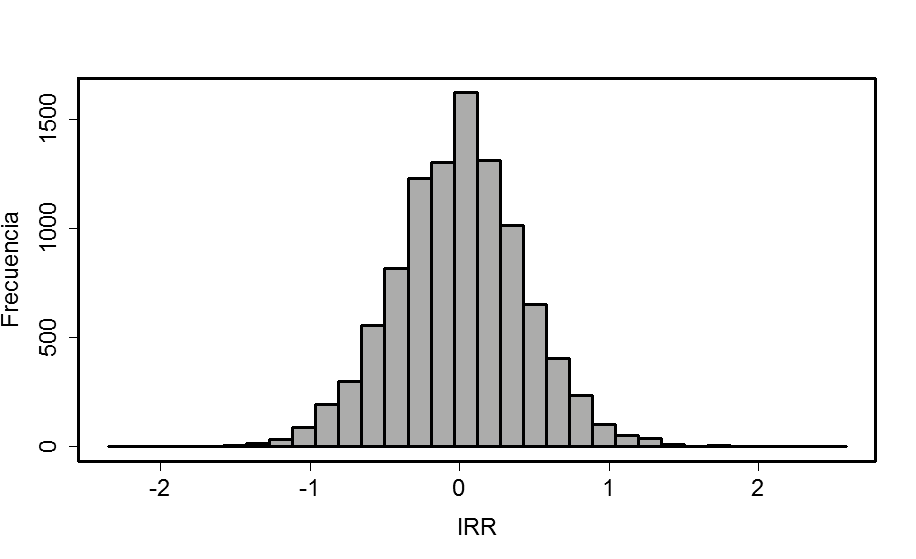
\includegraphics[width=13cm]{../fig/Cap09-EjemploLogRR02-bn.png}
\end{bn}
\caption{Simulación con $10000$ muestras, de tamaño $n=50$, con $p_1=p_2=0.2$, en el Ejemplo \ref{cap09:ejem:TransformandoRiesgoRelativoConLogaritmos}. (a) Distribución muestral  del riesgo relativo. (b) Distribución muestral del {\bf logaritmo} del riesgo relativo.}
\label{cap06:fig:EjemploLogRR01}
\end{center}
\end{figure}

Como puede verse en la figura, se obtiene una distribución muestral de $\widehat{RR}$ con el máximo en $1$, como esperábamos, pero muy asimétrica: con una cola derecha muy larga (debida a los cocientes $\frac{p_1}{p_2}$, en los que $p_2$ es muy pequeño comparado con $p_1$), mientras que la cola izquierda apenas existe, porque el riesgo relativo no puede tomar valores negativos. En estas condiciones, aproximar esta distribución por una normal no estaría justificado.

La idea es muy sencilla, pero es uno de esos ``trucos del oficio'' que resultan difíciles de justificar a priori. Digamos, por el momento, que es una buena idea, que funciona, y después trataremos de ver la lógica que se esconde detrás. Lo que vamos a hacer es tomar el logaritmo del riesgo relativo. Es decir, que para cada una de las $10000$ muestras, calculamos el número:
\[ln(\widehat{RR})=\ln\left(\dfrac{\hat p_1}{\hat p_2}\right)=\ln(\hat p_1)-\ln(\hat p_2).\]
El histograma de esos $10000$ logaritmos aparece en la parte (b) de la Figura \ref{cap06:fig:EjemploLogRR01}. Y, como puede verse, esa distribución se parece mucho más a una distribución normal.

Como hemos dicho antes, el lector puede preguntarse hasta qué punto estos resultados dependen de los valores concretos de $p_1$ y $p_2$, o del tamaño de muestra $n=50$ que hemos elegido. Gracias al Teorema Central del Límite (aunque en este caso su intervención no resulta tan evidente), si mantenemos $p_1=p_2=0.2$, pero aumentamos el tamaño de las muestras hasta $n=250$, entonces la distribución de los propios valores de $\widehat{RR}$ se acerca más a la normalidad, como puede verse en la parte (a) de la Figura \ref{cap06:fig:EjemploLogRR02}. Pero, si tomamos logaritmos, la normalidad mejora, también en este caso, como puede verse en la parte (b) de esa Figura.

El caso que estamos examinando en este ejemplo, en el que $p_1=p_2$, implica que los valores observados de $\widehat{RR}$ se concentren en torno a $1$. Pero los valores anormalmente pequeños de $p_2$ (que está en el denominador de $\widehat{RR}$) producen valores grandes de $\widehat{RR}$. Eso contribuye a explicar que la cola derecha de la distribución de $\widehat{RR}$ sea tan larga.  Podemos preguntarnos que sucedería si los dos valores fueran cercanos a $1$, o si $p_1$ y $p_2$ fueran muy distintos. Este segundo caso, con $p_1=0.2$ y $p_2=0.8$, se ilustra en la Figura \ref{cap06:fig:EjemploLogRR03} (pág. \pageref{cap06:fig:EjemploLogRR03}), que permite comprobar que tomar logaritmos no es la {\em panacea universal}, que resuelva nuestros problemas con las distribuciones que no son normales. En esa figura puedes comprobar que de hecho, la distribución de $\widehat{RR}$ se parecía más a un normal, que la que se obtiene para $\ln(\widehat{RR})$.  Como hemos dicho, en el Tutorial09, cuando veamos el código con el que se han generado estas simulaciones, podrás experimentar con otros tamaños de muestra, y con combinaciones de distintas de los valores $p_1$ y $p_2$.
\begin{figure}[p]
\begin{center}
\begin{enColor}
(a)\\[3mm]
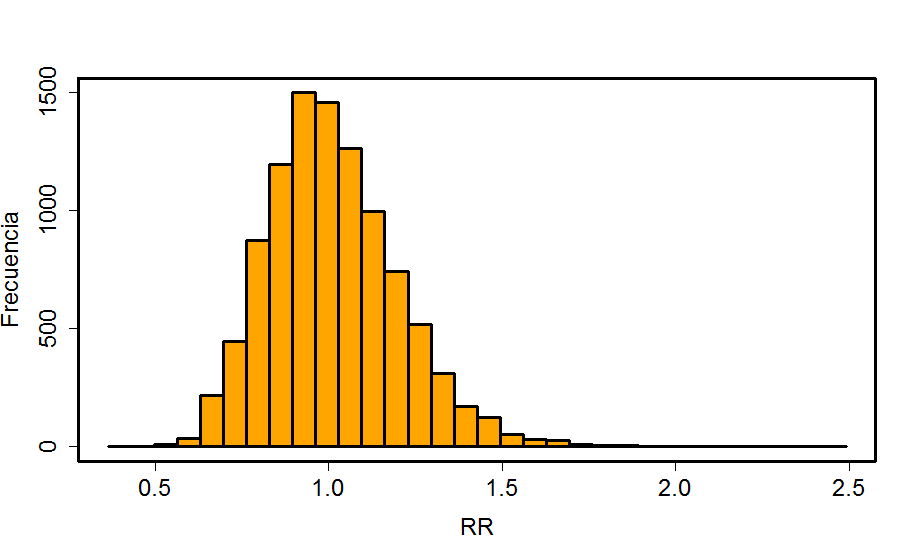
\includegraphics[width=13cm]{../fig/Cap09-EjemploLogRR03.png}\\[3mm]
(b)\\[3mm]
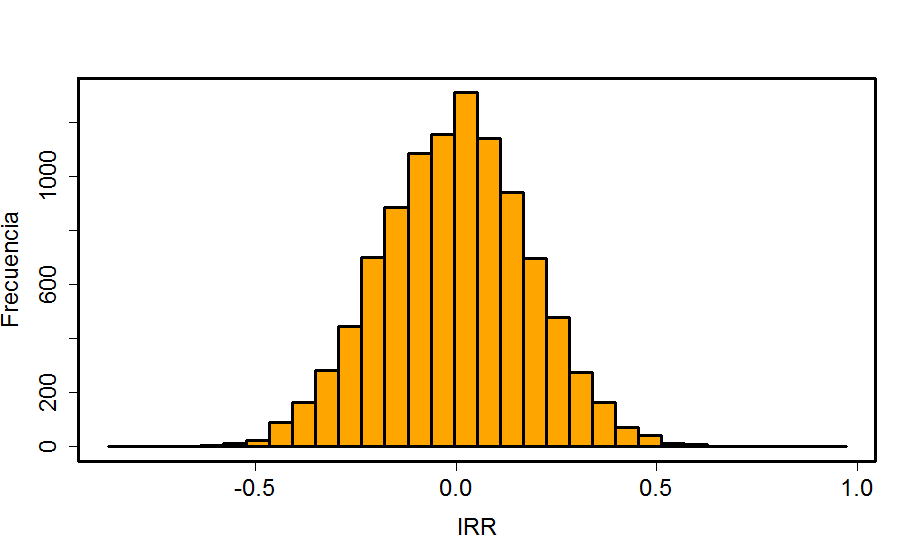
\includegraphics[width=13cm]{../fig/Cap09-EjemploLogRR04.png}
\end{enColor}
\begin{bn}
(a)\\[3mm]
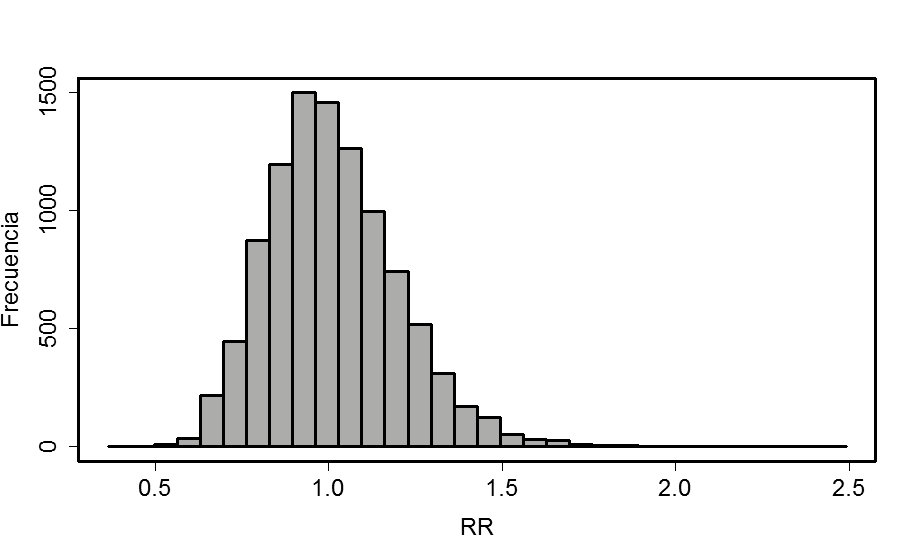
\includegraphics[width=13cm]{../fig/Cap09-EjemploLogRR03-bn.png}\\[3mm]
(b)\\[3mm]
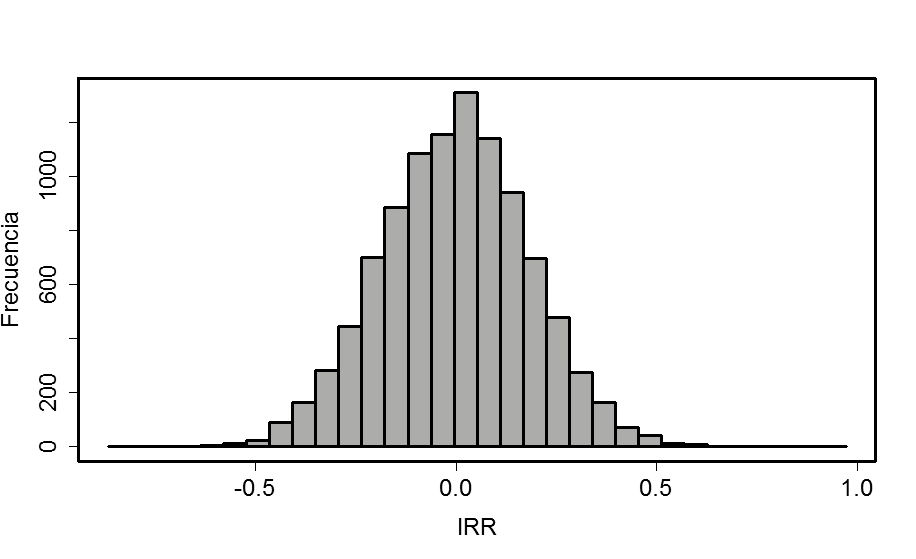
\includegraphics[width=13cm]{../fig/Cap09-EjemploLogRR04-bn.png}
\end{bn}
\caption{Simulación con $10000$ muestras, de tamaño $n=250$, con $p_1=p_2=0.2$, en el Ejemplo \ref{cap09:ejem:TransformandoRiesgoRelativoConLogaritmos}. (a) Distribución muestral  del riesgo relativo. (b) Distribución muestral del {\bf logaritmo} del riesgo relativo.}
\label{cap06:fig:EjemploLogRR02}
\end{center}
\end{figure}

\begin{figure}[p]
\begin{center}
\begin{enColor}
(a)\\[3mm]
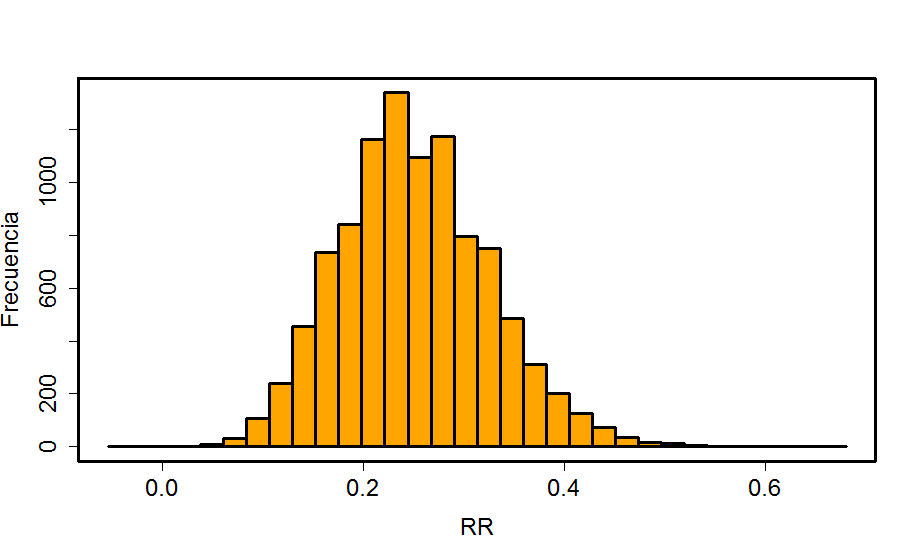
\includegraphics[width=13cm]{../fig/Cap09-EjemploLogRR05.png}\\[3mm]
(b)\\[3mm]
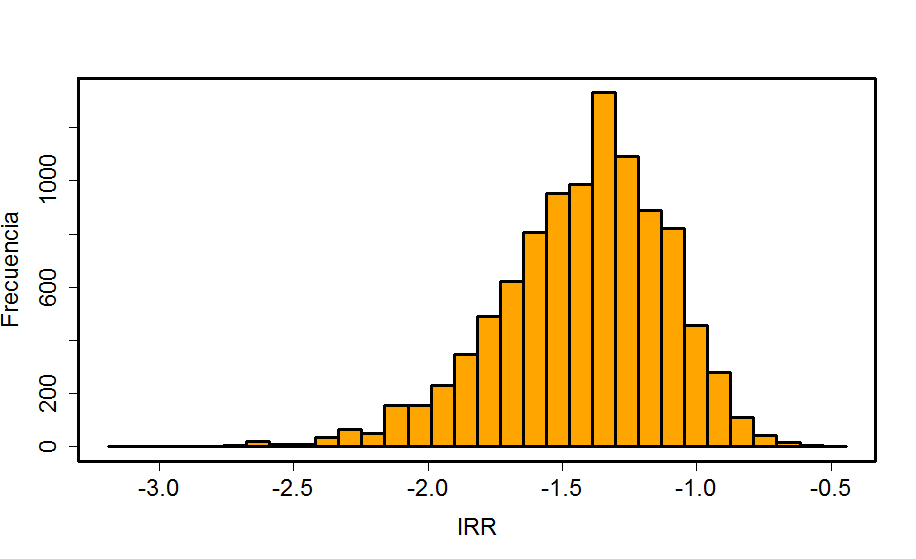
\includegraphics[width=13cm]{../fig/Cap09-EjemploLogRR06.png}
\end{enColor}
\begin{bn}
(a)\\[3mm]
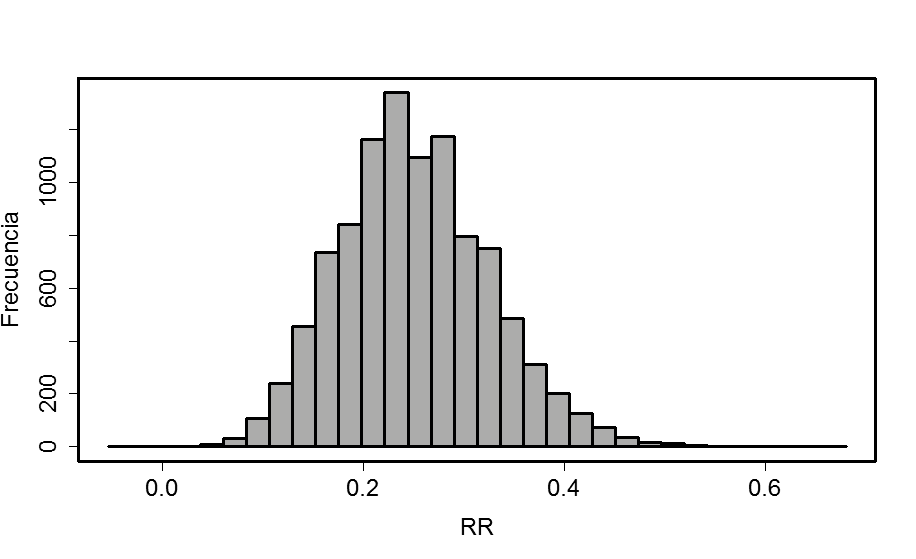
\includegraphics[width=13cm]{../fig/Cap09-EjemploLogRR05-bn.png}\\[3mm]
(b)\\[3mm]
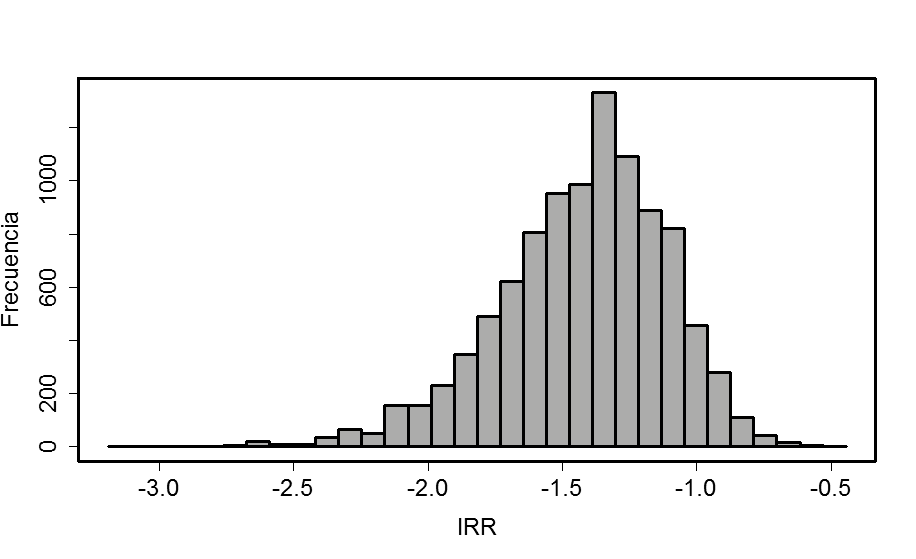
\includegraphics[width=13cm]{../fig/Cap09-EjemploLogRR06-bn.png}
\end{bn}
\caption{Simulación con $10000$ muestras, de tamaño $n=50$, con $p_1=0.2$ y $p_2=0.8$, en el Ejemplo \ref{cap09:ejem:TransformandoRiesgoRelativoConLogaritmos}. (a) Distribución muestral  del riesgo relativo. (b) Distribución muestral del {\bf logaritmo} del riesgo relativo.}
\label{cap06:fig:EjemploLogRR03}
\end{center}
\end{figure}
\qed
\end{ejemplo}

En algunos casos, como ilustra el Ejemplo \ref{cap09:ejem:TransformandoRiesgoRelativoConLogaritmos},  tenemos una muestra
\[x_1,\,x_2,\,\ldots,x_k\]
de una variable aleatoria $X$, que sólo toma valores positivos, con una distribución asimétrica en la que la cola derecha es muy larga. En tal caso podemos {\sf transformar}\index{transformación de variables aleatorias} la variable aleatoria, definiendo
\begin{equation}
\label{cap09:ecu:TransformacionVariablesConLogaritmo}
Y=\ln(X)
\end{equation}
Y, como muestra ese ejemplo, a veces la variable $Y$ tiene una distribución más parecida a la normal que la la variable original $X$. En esos casos resulta ventajoso realizar inferencia {\em sobre los valores de la variable $Y$}. Es muy importante prestar atención a esta última frase: la inferencia se hace sobre los valores de $Y$, no sobre los valores de $X$, así que nuestras conclusiones hablarán de $Y$, en lugar de $X$.


¿Por qué tomar logaritmos?  Sin ponernos demasiado técnicos, la Figura
\ref{cap09:fig:LogaritmoComoTransformacion} pretende ayudar a entender el efecto de tomar
logaritmos sobre un conjunto de datos. Hemos dibujado con trazo continuo (en azul, si estás mirando
una copia en color) la parte de la gráfica del logaritmo, $y=\ln x$, que corresponde a valores
$0<x<1$. Como puedes ver, ese intervalo $0<x<1$, se ``estira'' a través del logaritmo, para
convertirse en el intervalo $(-\infty,0)$. Por otra parte, como indica el trazo discontinuo (en
azul), el conjunto de valores $x>1$ se convierte, mediante el logaritmo, en el intervalo
$(0,\infty)$, pero de tal forma que los valores muy grandes de $x$ producen valores sólo
moderadamente grandes de $y$. Los valores cercanos a $1$ son los que menos transformación
experimentan.

\begin{figure}[htb]
\begin{center}
\begin{enColor}
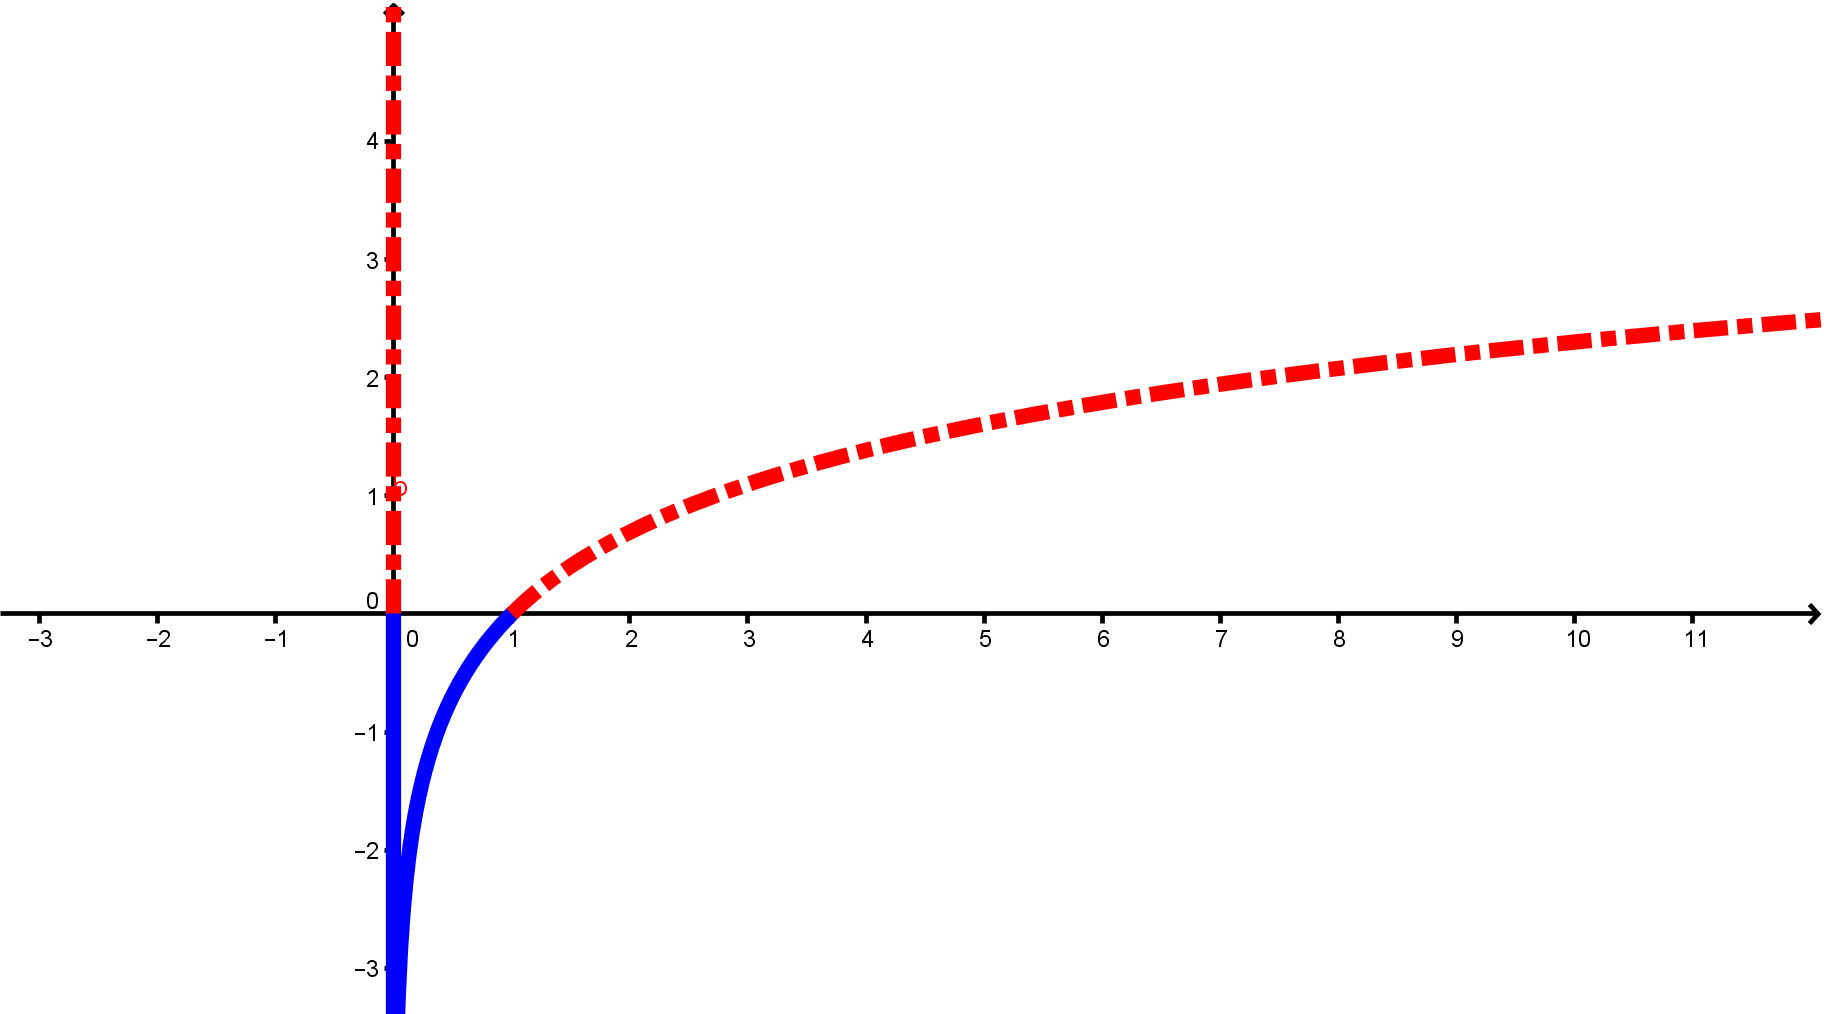
\includegraphics[width=13.5cm]{../fig/Cap09-TransformacionDatosConLogaritmo.png}
\end{enColor}
\begin{bn}
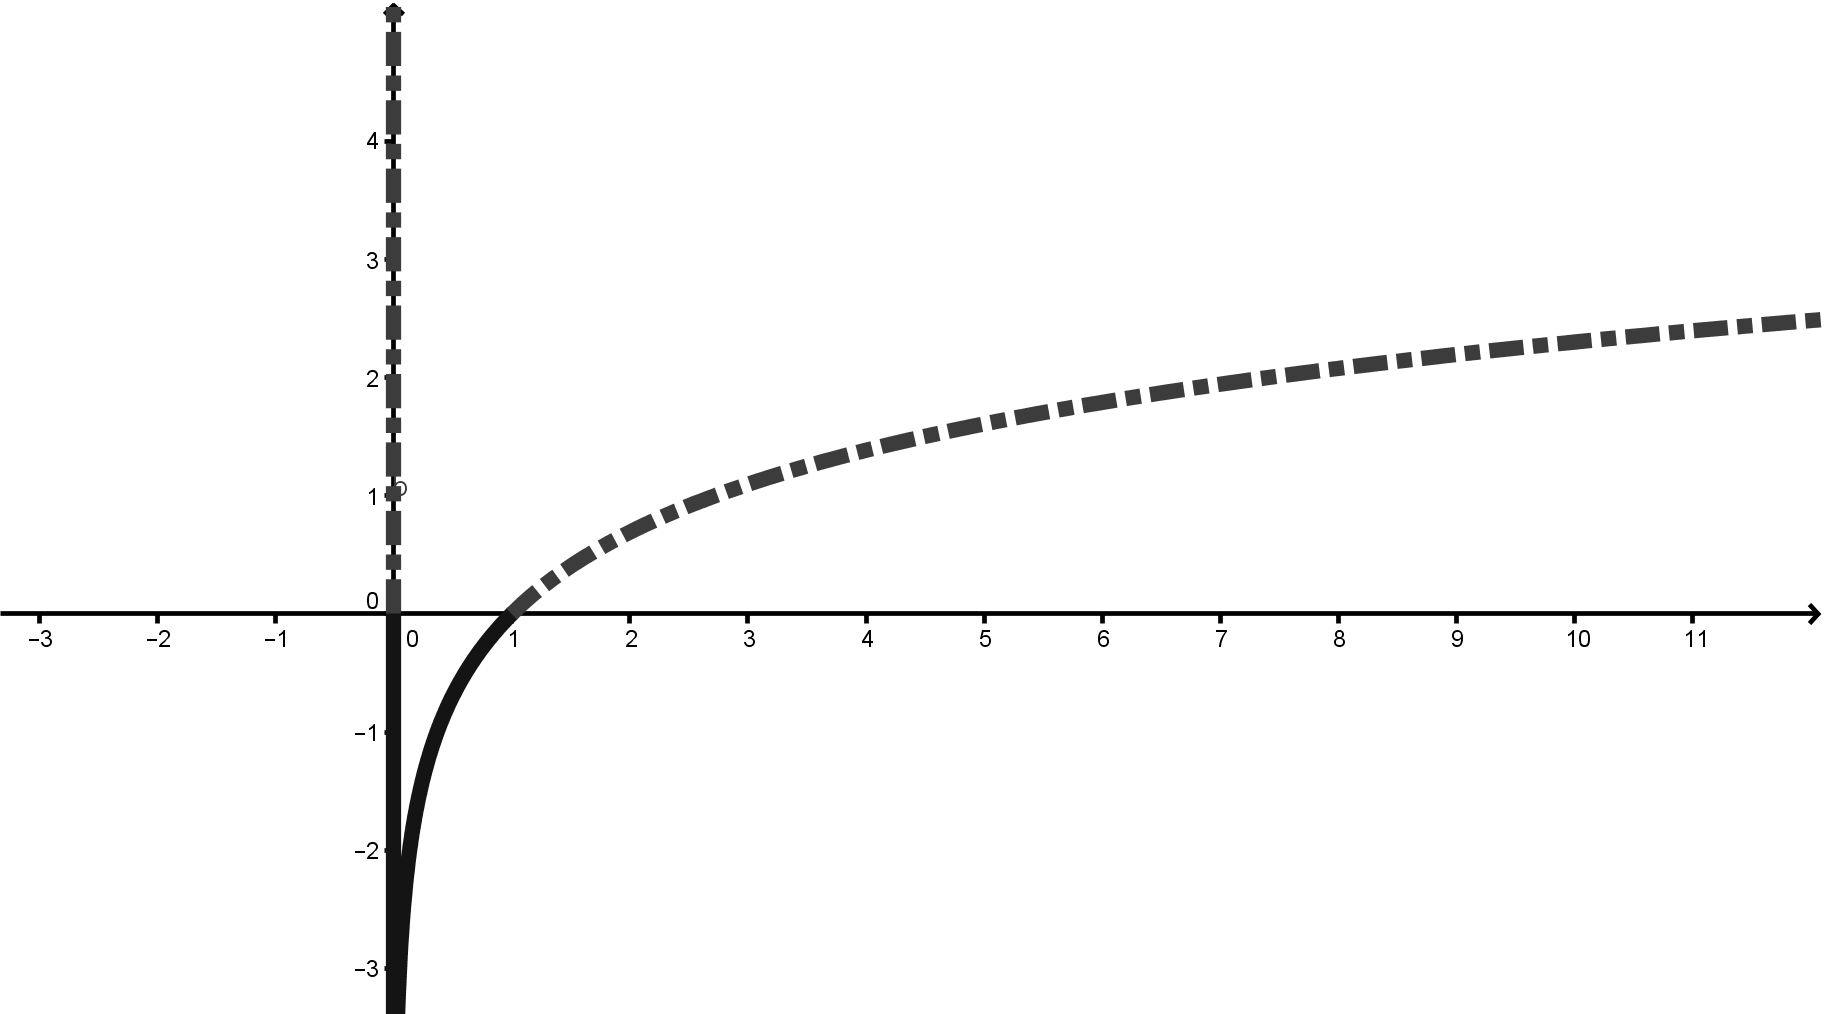
\includegraphics[width=13.5cm]{../fig/Cap09-TransformacionDatosConLogaritmo-bn.png}
\end{bn}
\caption{El logaritmo, y su efecto como transformación de datos.}
\label{cap09:fig:LogaritmoComoTransformacion}
\end{center}
\end{figure}

A los matemáticos a menudo les ayuda pensar en el logaritmo, y en otras funciones, de esta manera, en la que los intervalos se ``estiran'', o ``contraen'' y, en general, se ``deforman'' de alguna manera que pueda resultarnos útil. Vimos un ejemplo parecido al hablar de posibilidades (odds), en la página \pageref{cap12:Fig:OddsVsProbabilidad}. Fíjate, en particular, en la Figura \ref{cap12:Fig:OddsVsProbabilidad} de esa página, en la que mostrábamos que las posibilidades se podían entender como un cambio de escala, o transformación (en nuestro lenguaje actual), de las probabilidades. Esta reinterpretación de las posibilidades va a jugar un papel importante dentro de un momento, en esta misma sección. Y volviendo a la discusión del Ejemplo \ref{cap09:ejem:TransformandoRiesgoRelativoConLogaritmos}, si piensas un poco sobre el logaritmo, desde esta perspectiva, comprenderás porque puede ser una transformación útil cuando tenemos mucha probabilidad acumulada cerca del origen, y queremos repartirla de una forma más parecida a la normal.

No vamos a entrar siquiera a discutir cuándo y cómo podemos (o debemos) transformar los datos. Y no lo haremos por dos razones. En primer lugar, porque el tema de la transformación de variables aleatorias es muy sutil, y  sólo podemos limitarnos a rozar la superficie. Recomendamos, en cualquier caso, al lector interesado, la lectura de la Sección 4.3 del libro de Quinn y Keough (referencia \cite{quinn2002experimental} en la Bibliografía).

En segundo lugar, porque, para justificar la transformación, hemos dicho que lo hacíamos para obtener una distribución más aproximada a la normal y, de esa forma, ser capaces de usar los métodos de inferencia que hemos visto y que, en su gran mayoría, se apoyan en
%alguna variante del TCL (y por tanto, en
la suposición de que los datos son, al menos aproximadamente, normales. Y hay, desde luego, otra salida, aparte de la transformación, cuando nuestros datos no cumplen la hipótesis de normalidad: usar métodos de inferencia que no necesiten esa hipótesis. Hay bastantes métodos de esta clase, de los llamados {\sf métodos no paramétricos}, que no asumen que los datos de partida sean aproximadamente normales. Hablaremos más sobre esos métodos no paramétricos en el Apéndice \ref{apendice:MasAlla} (pág. \pageref{apendice:MasAlla}).

\subsubsection{Variable lognormal}
\label{cap09:subsubsec:VariableLogNormal}

Hemos visto que existen variables aleatorias cuyo logaritmo se comporta, aproximadamente, como una distribución normal. No queremos desaprovechar la oportunidad para comentar que existe un modelo teórico de este tipo de variables aleatorias, las llamadas {\sf variables lognormales}.

\begin{center}
    \fcolorbox{black}{Gris025}{
    \begin{minipage}{12.5cm}
        %%%%%%%%%%%%%%%%%%%%%%%%%%%%%%%%%%%%%%%
        \begin{center}
        {\bf Variable aleatoria lognormal.}
        \index{variable aleatoria lognormal}\index{lognormal, variable aleatoria}
        \end{center}
       %%%%%%%%%%%%%%%%%%%%%%%%%%%%%%%%%%%%%%%
       Una variable aleatoria $X$ es de tipo {\sf lognormal} con media $\mu$ y desviación típica $\sigma$ si se cumple:
       \begin{equation}
       \label{cap09:ecu:VariableLogNormal}
       \ln(X)\sim N(\mu,\sigma)
       \end{equation}
       %%%%%%%%%%%%%%%%%%%%%%%%%%%%%%%%%%%%%%%
    \end{minipage}}
\end{center}
En el Tutorial09 veremos como usar el ordenador para trabajar con estas variables.


\subsection{Inferencia sobre el riesgo relativo y el cociente de posibilidades.}
\label{cap09:subsec:InferenciaRiesgoRelativo}

Ahora que ya hemos discutido, siquiera brevemente, las razones por las que puede ser conveniente considerar como variable de interés el logaritmo del riesgo relativo:
\[\ln(RR)=\ln\left(\dfrac{\hat p_1}{\hat p_2}\right),\]
lo que necesitamos es información muestral sobre esta cantidad.

\begin{center}
    \fcolorbox{black}{Gris025}{
    \begin{minipage}{12.5cm}
        %%%%%%%%%%%%%%%%%%%%%%%%%%%%%%%%%%%%%%%
        \begin{center}
        {\bf Intervalo de confianza para el logaritmo del riesgo relativo.}
        \index{intervalo de confianza para el logaritmo del riesgo relativo}
        \index{riesgo relativo, intervalo de confianza para su logaritmo}
        \end{center}
       %%%%%%%%%%%%%%%%%%%%%%%%%%%%%%%%%%%%%%%
        Supongamos que hemos tomado muestras de tamaños $n_1$ y $n_2$, respectivamente, de dos poblaciones independientes, ambas de tipo Bernouilli, con proporciones de éxito iguales, respectivamente, a $p_1$ y $p_2$. Supongamos, además, que se cumplen las condiciones \ref{cap09:ecu:CondicionesInferenciaDiferenciaProporciones} (pág. \pageref{cap09:ecu:CondicionesInferenciaDiferenciaProporciones}) para aproximar las binomiales por normales. Entonces un intervalo de confianza al nivel $nc=1-\alpha$ para el {\sf logaritmo del riesgo relativo} $\ln(RR)$ es:
        \begin{equation}
        \label{cap09:ecu:IntConfRiesgoRelativo}
        \ln(RR)=\ln\left(\dfrac{\hat p_1}{\hat p_2}\right)\pm z_{\alpha/2}\sqrt{\dfrac{\hat q_1}{n_1\hat p_1}+\dfrac{\hat q_2}{n_2\hat p_2}},
       \end{equation}
       donde $\hat q_i=1-\hat p_i$, para $i=1,2$.
       %%%%%%%%%%%%%%%%%%%%%%%%%%%%%%%%%%%%%%%
    \end{minipage}}
\end{center}

Es habitual, después de calcular un intervalo de confianza para $\ln(RR)$ usando la Ecuación \ref{cap09:ecu:IntConfRiesgoRelativo}, calcular la exponencial de los extremos de ese intervalo, para obtener un intervalo para $RR$.

¿De dónde ha salido la raíz cuadrada que hemos usado para construir este intervalo de confianza? Las expresiones de la semianchura de un intervalo de confianza, como la de la Ecuación \ref{cap09:ecu:IntConfRiesgoRelativo}, se obtienen en casos como este, con relativa facilidad, utilizando el conocido como {\sf método $\delta$ (delta)}\index{método delta}\index{delta, método}. Este método permite encontrar el error estándar en situaciones como esta, en las que se ha aplicado una transformación a una variable aleatoria, como hemos hecho aquí con el logaritmo. El lector interesado puede encontrar una descripción del método delta en la pág. 593 del libro de B.Rosner (referencia \cite{rosner2011fundamentals} en la Bibliografía).

Con frecuencia, en lugar del riesgo relativo, que es el cociente de probabilidades, se utiliza como alternativa otro cociente, el {\sf cociente de posibilidades}\index{cociente de posibilidades}\index{posibilidades, cociente} (en inglés, {\em odds ratio}\index{odds ratio}, a menudo abreviado como $OR$\index{$OR$, odds ratio}), definido mediante (se usan posibilidades {\em a favor}):
\begin{equation}
\label{cap09:ecu:DefinicionOddsRatio}
OR=\dfrac{O_1}{O_2}=\dfrac{\phantom{a}\left(\dfrac{p_1}{q_1}\right)\phantom{a}}{\left(\dfrac{p_2}{q_2}\right)}
\end{equation}
El estimador natural para $OR$ es, por supuesto, el {\em cociente de posibilidades muestrales}:
\[
\widehat{OR}=
\dfrac{\hat O_1}{\hat O_2}=
\dfrac{\phantom{a}\left(\dfrac{\hat p_1}{\hat q_1}\right)\phantom{a}}
{\left(\dfrac{\hat p_2}{\hat q_2}\right)}.
\]
Vamos a utilizar el lenguaje de las tablas de contingencia para expresar este estimador, porque así se obtiene una expresión particularmente sencilla, y porque (en consecuencia) ese es el lenguaje habitual en las aplicaciones. Supongamos que la información de las dos muestras se recoge en una Tabla como la \ref{cap09:tabla:notacionTablaContingenciaContrasteProporciones}, en la que los valores indican el número de observaciones (que son números enteros), en lugar de las proporciones muestrales (que son fracciones). Así, por ejemplo, $n_{12}$ es el número de éxitos observados en la población $2$.

\begin{table}[ht]
        \begin{center}
        \begin{tabular}{cc|c|c|c|}
              &\multicolumn{1}{c}{}&\multicolumn{3}{c}{}\\
              \cline{3-5}
              % after \\: \hline or \cline{col1-col2} \cline{col3-col4} ...
               &\multicolumn{1}{c|}{}& Población $1$&  Población $2$ & Total \\
               \cline{2-5}
        &\multicolumn{1}{|c|}{Éxitos}& $n_{11}$ & $n_{12}$ & $n_{1+}=n_{11}+n_{12}$ \\ % 11 8 19
              \cline{2-5}
             & \multicolumn{1}{|c|}{Fracasos}& $n_{21}$ & $n_{22}$ &  $n_{2+}=n_{21}+n_{22}$\\ % 4  7 11
              \cline{2-5}
             & \multicolumn{1}{|c|}{Total} & $n_{+1}=n_{11}+n_{21}$ & $n_{+2}=n_{12}+n_{22}$ & $n$ \\
              \cline{2-5}
        \end{tabular}
        \end{center}
\caption{Tablas de contingencia para un contraste de proporciones.}
\label{cap09:tabla:notacionTablaContingenciaContrasteProporciones}
\end{table}
Con la notación de la Tabla \ref{cap09:tabla:notacionTablaContingenciaContrasteProporciones}, el estimador de $OR$ se escribe así (en la segunda igualdad, hemos cancelado todos los denominadores $n$):
\begin{equation}
\label{cap09:ecu:EstimadorMuestralORconTablaContingencia}
\widehat{OR}=\dfrac{\hat O_1}{\hat O_2}=
\dfrac{\phantom{a}\left(\dfrac{\hat p_1}{\hat q_1}\right)\phantom{a}}
{\left(\dfrac{\hat p_2}{\hat q_2}\right)}=
\dfrac{\phantom{a}\left(\dfrac{n_{11}}{n_{21}}\right)\phantom{a}}
{\left(\dfrac{n_{12}}{n_{22}}\right)}=\dfrac{n_{11}\cdot n_{22}}{n_{12}\cdot n_{21}}
\end{equation}
Y, como puede verse, el estimador es simplemente el cociente de los productos de las dos diagonales (principal en el numerador, secundaria en el denominador) de la matriz:
\begin{equation}
\label{cap09:ecu:Matriz2x2InferenciaOR}
\left(
\vcenter{
\xymatrix{
n_{11}\ar@{<->}[dr]&n_{12}\\
n_{21}\ar@{<->}[ur]&n_{22}
}
}
\right)
\end{equation}

De nuevo, como hemos visto que sucedía con el cociente de probabilidades, para hacer inferencia se utiliza preferentemente el logaritmo de $OR$, porque su distribución es, en general, más ajustada a una curva normal que la del propio cociente $OR$. Además, cuando se usa el logaritmo, el término de error que interviene en la expresión del intervalo de confianza se puede escribir de forma muy sencilla, a partir de los elementos de la matriz  \ref{cap09:ecu:Matriz2x2InferenciaOR}. Usando el método delta del que hemos hablado antes, se obtiene esa expresión.

\begin{center}
    \fcolorbox{black}{Gris025}{
    \begin{minipage}{12.5cm}
        %%%%%%%%%%%%%%%%%%%%%%%%%%%%%%%%%%%%%%%
        \begin{center}
        {\bf Intervalo de confianza para el logaritmo del cociente de posibilidades (odds ratio).}
        \index{intervalo de confianza para el logaritmo del cociente de posibilidades (odds ratio)}
        \index{cociente de posibilidades (odds ratio), intervalo de confianza para su logaritmo}
        \end{center}
       %%%%%%%%%%%%%%%%%%%%%%%%%%%%%%%%%%%%%%%
        Como antes, supongamos que hemos tomado muestras de tamaños $n_1$ y $n_2$, respectivamente, de dos poblaciones independientes, ambas de tipo Bernouilli, con proporciones de éxito iguales, respectivamente, a $p_1$ y $p_2$. Supongamos, además, que se cumplen las condiciones \ref{cap09:ecu:CondicionesInferenciaDiferenciaProporciones} (pág. \pageref{cap09:ecu:CondicionesInferenciaDiferenciaProporciones}) para aproximar las binomiales por normales. Entonces un intervalo de confianza al nivel $nc=1-\alpha$ para el {\sf logaritmo del cociente de posibilidades (odds ratio)} $\ln(OR)$ es:
        \begin{equation}
        \label{cap09:ecu:IntConfLogaritmoOR}
        \ln(OR)=
        \ln\left(\dfrac{n_{11}\cdot n_{22}}{n_{12}\cdot n_{21}}\right)\pm z_{\alpha/2}
        \sqrt{\dfrac{1}{n_{11}}+\dfrac{1}{n_{12}}+\dfrac{1}{n_{21}}+\dfrac{1}{n_{22}}}
       \end{equation}
       %%%%%%%%%%%%%%%%%%%%%%%%%%%%%%%%%%%%%%%
    \end{minipage}}
\end{center}
La fórmula para la semianchura del intervalo se obtiene de nuevo aplicando el {\em método delta} al que aludíamos antes. Dentro de la raíz cuadrada aparece simplemente la suma de los inversos de todos los elementos de la matriz \ref{cap09:ecu:Matriz2x2InferenciaOR}. Al igual que en el caso del riesgo relativo, se puede calcular la exponencial de los extremos de este intervalo, y así obtener un intervalo para el cociente de posibilidades.

Una propiedad interesante del cociente de posibilidades es que, como puede verse en la Ecuación \ref{cap09:ecu:IntConfLogaritmoOR}, el intervalo de confianza es el mismo si se cambian filas por columnas. Es decir, que la estimación de $OR$ no depende de que escribamos la población en las columnas y el tratamiento en las filas o viceversa. Volveremos a encontrarnos con esta simetría en el Capítulo \ref{cap:TablasContingenciaTestChi2}, donde examinaremos este mismo problema del contraste de proporciones entre dos poblaciones usando otros puntos de vista.

Cerraremos esta sección con un ejemplo.
\begin{ejemplo}
\label{cap09:ejem:PruebasDiagnosticasInferencia_OR_RR}
En la Tabla \ref{cap03:tabla:ejemploPruebasDiagnosticas} (pág. \pageref{cap03:tabla:ejemploPruebasDiagnosticas}) hemos visto un ejemplo de tabla de contingencia para una prueba diagnóstica, que por comodidad reproducimos aquí como Tabla \ref{cap09:tabla:ejemploPruebasDiagnosticas}.

\begin{table}[h!]
        \begin{center}
            \begin{tabular}{llccc}
            &&\multicolumn{3}{c}{\underline{\bf Padecen la enfermedad}}\\

                                      &          & Sí &  No & Total\\
            \hline
          \underline{\bf Diagnóstico} & Positivo & 192&  158&   350\\
                                      & Negativo &  4 & 9646&  9650\\
            \cline{2-5}
                                      & Total    & 196& 9804& 10000\\
            \hline
            \end{tabular}
        \end{center}
        \caption{Tabla de contingencia del Ejemplo \ref{cap09:ejem:PruebasDiagnosticasInferencia_OR_RR}}
        \label{cap09:tabla:ejemploPruebasDiagnosticas}
\end{table}
Empecemos calculando las estimaciones muestrales de las proporciones de éxitos y fracasos para ambas poblaciones:
\[
\begin{cases}
    \hat p_1=\dfrac{192}{196}\approx 0.9796\\[3mm]
    \hat q_1=\dfrac{4}{196}\approx 0.02041\\[3mm]
    \hat p_2=\dfrac{158}{9804}\approx 0.01612\\[3mm]
    \hat q_2=\dfrac{9646}{9804}=0.9839
\end{cases}
\quad
\mbox{, y por tanto }
\quad
\begin{cases}
    \hat O_1=\dfrac{192}{4}=48\\[3mm]
    \hat O_2=\dfrac{158}{9646}\approx 0.01638
\end{cases}
\]
A partir de aquí es fácil usar la Ecuación \ref{cap09:ecu:IntConfRiesgoRelativo} para obtener un intervalo de confianza al $95\%$ para $\ln(RR)$:
\[
\ln(RR)=\ln\left(\dfrac{0.9796}{0.01612}\right)\pm z_{\alpha/2}\sqrt{\dfrac{0.02041}{196\cdot 0.9796}+\dfrac{0.9839}{9804\cdot 0.01612}},
\]
es decir, aproximadamente:
\[
\ln(RR)=4.107\pm 0.1560,\mbox{ o, lo que es lo mismo } 3.952<\ln(RR)<4.264
\]
Calculando las exponenciales de los extremos del intervalo se obtiene, para el riesgo relativo:
\[52< RR < 71\mbox { con }\widehat{RR}\approx 60.78.\]

Vamos ahora a calcular un intervalo de confianza para el logaritmo del cociente de posibilidades (odds ratio). El estimador muestral de $OR$ es:
\[\widehat{OR} = \dfrac{192\cdot 9646}{4\cdot 158}\approx 2930.\]
Y el intervalo de confianza para $\ln(OR)$ es, según la Ecuación \ref{cap09:ecu:IntConfLogaritmoOR}:
\[
        \ln(OR)\approx
        \ln\left(2930\right)\pm z_{\alpha/2}
        \sqrt{\dfrac{1}{192}+\dfrac{1}{158}+\dfrac{1}{4}+\dfrac{1}{9646}},
\]
es decir:
\[
\ln(OR)\approx 7.983\pm 1.003,\mbox{ o, lo que es lo mismo } 6.980<\ln(OR)<8.985
\]
Calculando las exponenciales de los extremos del intervalo se obtiene, para el cociente de posibilidades:
\[1075< OR < 7986, \quad \mbox {con } OR\approx 2930.\]
Este resultado se interpreta como que las posibilidades a favor de padecer la enfermedad, tras un resultado positivo en el test, son de 2930 a 1, cuando se compara la población enferma con la sana.  Redondeando, $3000$ a $1$.

Sin entrar en detalles, usando los métodos de la Sección \ref{cap09:sec:DiferenciaProporciones2Poblaciones} (ver la Ecuación \ref{cap09:ecu:IntConfDiferenciaProporciones}, pág. \pageref{cap09:ecu:IntConfDiferenciaProporciones}), se puede calcular un intervalo de confianza para la {\em diferencia} de proporciones:
\[0.9435 < p_1-p_2 <0.9834\]
Pero, como puedes ver, puesto que la diferencia de tamaño de ambas proporciones es tan grande, seguramente resulta más informativo cualquiera de los otros dos intervalos de confianza (para el cociente de probabilidades o posibilidades) que hemos construido en este ejemplo. En particular, a nosotros nos resulta especialmente fácil de entender la información de que el riesgo relativo de dar positivo es, para un enfermo, aproximadamente $61$ veces mayor que para una persona sana.

\qed
\end{ejemplo}

Por supuesto, además de los intervalos de confianza, nos interesan los contrastes de hipótesis relativos a $RR$ y $OR$. O, más precisamente, a sus logaritmos. Ya sabemos que lo importante es conocer el estadístico relevante para cada caso.

\begin{center}
    \fcolorbox{black}{Gris025}{
    \begin{minipage}{12.5cm}
        %%%%%%%%%%%%%%%%%%%%%%%%%%%%%%%%%%%%%%%
        \begin{center}
        {\bf Estadísticos para contrastes sobre $RR$ y $OR$.}
        \end{center}
       %%%%%%%%%%%%%%%%%%%%%%%%%%%%%%%%%%%%%%%
        Si hemos tomado muestras de tamaños $n_1$ y $n_2$, respectivamente, de dos poblaciones independientes, ambas de tipo Bernouilli, con proporciones de éxito iguales, respectivamente, a $p_1$ y $p_2$, y se cumplen las condiciones \ref{cap09:ecu:CondicionesInferenciaDiferenciaProporciones} (pág. \pageref{cap09:ecu:CondicionesInferenciaDiferenciaProporciones}) para aproximar las binomiales por normales, entonces el estadístico adecuado para hacer contrastes sobre:
        \begin{itemize}
          \item el {\sf logaritmo del riesgo relativo} $\ln(RR)$ es:
            \begin{equation}
            \label{cap09:ecu:IntConfRiesgoRelativo}
            \dfrac{\ln\left(\dfrac{\hat p_1}{\hat p_2}\right)-\ln(RR)}{\sqrt{\dfrac{\hat q_1}{n_1\hat p_1}+\dfrac{\hat q_2}{n_2\hat p_2}}}\sim Z.
           \end{equation}

          \item el {\sf logaritmo del cociente de posibilidades (odds ratio)} $\ln(OR)$ es
            \begin{equation}
            \label{cap09:ecu:EstadisticoContrasteLogaritmoOR}
            \dfrac{\ln\left(\dfrac{n_{11}\cdot n_{22}}{n_{12}\cdot n_{21}}\right)-\ln(OR)}{
            \sqrt{\dfrac{1}{n_{11}}+\dfrac{1}{n_{12}}+\dfrac{1}{n_{21}}+\dfrac{1}{n_{22}}}}\sim Z.
           \end{equation}
        \end{itemize}
        En ambos casos, como se indica, los estadísticos se distribuyen según  la normal estándar $Z$.
       %%%%%%%%%%%%%%%%%%%%%%%%%%%%%%%%%%%%%%%
    \end{minipage}}
\end{center}
Es muy habitual que queramos contrastar la igualdad de las proporciones en ambas poblaciones. Hay que tener en cuenta que, si $p_1=p_2$, entonces $RR=1$ y $OR=1$.  En términos de $\ln(RR)$ y $\ln(OR)$, eso se traduce, respectivamente, en que querremos contrastar las hipótesis nulas:
\[H_0=\{\ln(RR)=0\},\]
para $RR$, y
\[H_0=\{\ln(OR)=0\},\]
para $OR$. En ese caso, las fórmulas de los numeradores de ambos estadísticos se simplifican, al desaparecer el segundo término.
